% Tesis: rachas secas en Chile continental (CR2MET vs ALADIN)
% Compilar en local:  cd tesis && tectonic main.tex
% Overleaf: subir el zip que genera ./empaquetar_overleaf.sh (compilador XeLaTeX)
\documentclass[12pt,a4paper,oneside]{report}

\usepackage{fontspec}
\usepackage[spanish,es-tabla,es-nodecimaldot]{babel}
\usepackage[margin=2.5cm]{geometry}
\usepackage{setspace}
\onehalfspacing
\usepackage{graphicx}
\graphicspath{{figuras/}{../paper_figuras/}}
\usepackage{longtable,booktabs,array,calc}
\usepackage{etoolbox}
\AtBeginEnvironment{longtable}{\small}
\usepackage{amsmath,amssymb}
\usepackage{xcolor}
\usepackage{newunicodechar}
\usepackage{caption}
\captionsetup{font=small,labelfont=bf}
\usepackage[round,authoryear]{natbib}
\usepackage[hidelinks]{hyperref}

% Caracteres Unicode que la fuente Latin Modern no trae
\newunicodechar{₀}{\ensuremath{_0}}
\newunicodechar{₁}{\ensuremath{_1}}
\newunicodechar{−}{\ensuremath{-}}
\newunicodechar{Δ}{\ensuremath{\Delta}}
\newunicodechar{≥}{\ensuremath{\geq}}
\newunicodechar{≈}{\ensuremath{\approx}}
\newunicodechar{→}{\ensuremath{\rightarrow}}
\newunicodechar{α}{\ensuremath{\alpha}}
\newunicodechar{∫}{\ensuremath{\int}}
\newunicodechar{²}{\ensuremath{^2}}

% Definiciones que necesita el LaTeX generado por pandoc
\makeatletter\define@key{Gin}{alt}{}\makeatother
\providecommand{\tightlist}{\setlength{\itemsep}{0pt}\setlength{\parskip}{0pt}}
\newlength{\cslhangindent}
\newcounter{none}

% Marcador de trabajo pendiente; \renewcommand a vacío para ocultarlos
\newcommand{\pendiente}[1]{{\color{red!70!black}\itshape [PENDIENTE: #1]}}

% Poner en false para compilar sin la hoja de ruta
\newif\ifhojaderuta
\hojaderutatrue

\begin{document}

\begin{titlepage}
  \centering
  \vspace*{2cm}
  {\Large Universidad \pendiente{nombre}}\\[0.5cm]
  {\large Programa \pendiente{nombre}}\\[3cm]
  {\LARGE\bfseries Rachas secas en Chile continental:\\[0.3cm]
   evaluación de un modelo regional y cambios proyectados\par}
  \vspace{1cm}
  {\large \pendiente{título definitivo por acordar}}\\[3cm]
  {\large Tesis para optar al grado de \pendiente{grado}}\\[2cm]
  {\large Pablo Gómez}\\[0.5cm]
  {\large Profesor guía: \pendiente{nombre}}\\[2cm]
  {\large Santiago, \pendiente{fecha}}
\end{titlepage}

\pagenumbering{roman}
\ifhojaderuta
  \chapter*{Hoja de ruta: qué falta para la tesis y cómo abordarlo}
\addcontentsline{toc}{chapter}{Hoja de ruta}
\emph{Esta sección es de trabajo y se borra en la versión final. El resto del documento es el paper copiado (texto normal) más la estructura de tesis; lo que falta está marcado como} \textbf{\pendiente{\ldots{}}}.

\section*{A. Antes de escribir: definir con el profesor}\label{a.-antes-de-escribir-definir-con-el-profesor}
\addcontentsline{toc}{section}{A. Antes de escribir: definir con el profesor}

\begin{enumerate}
\def\labelenumi{\arabic{enumi}.}
\tightlist
\item
  \textbf{Reglamento y formato del programa.} Extensión, estructura obligatoria, idioma del resumen, estilo de citas, portada y márgenes. \emph{Cómo:} pedir el reglamento o una plantilla de tesis del programa y ajustar este draft a esa estructura.
\item
  \textbf{Dónde van las pruebas de sensibilidad.} En el paper están en el material suplementario; en la tesis pueden ir en el cuerpo (secciones de robustez en los capítulos 4 y 5) o en un anexo. \emph{Cómo:} proponer cuerpo para S1 (umbral) y S6 (escenario) y anexo para el resto; confirmar con el profesor.
\item
  \textbf{Hipótesis.} Decidir si el programa exige hipótesis formales; hay un borrador en §1.2.
\item
  \textbf{Alcance adicional.} Decidir si se agregan las PDFs por cuenca con SSP3-7.0 o se deja SSP3-7.0 solo en los risk ratios.
\end{enumerate}

\section*{B. Contenido nuevo que la tesis necesita (el paper no lo tiene)}\label{b.-contenido-nuevo-que-la-tesis-necesita-el-paper-no-lo-tiene}
\addcontentsline{toc}{section}{B. Contenido nuevo que la tesis necesita (el paper no lo tiene)}

{\def\LTcaptype{none} % do not increment counter
\begin{longtable}[]{@{}
  >{\raggedright\arraybackslash}p{(\linewidth - 6\tabcolsep) * \real{0.2500}}
  >{\raggedright\arraybackslash}p{(\linewidth - 6\tabcolsep) * \real{0.2500}}
  >{\raggedright\arraybackslash}p{(\linewidth - 6\tabcolsep) * \real{0.2500}}
  >{\raggedright\arraybackslash}p{(\linewidth - 6\tabcolsep) * \real{0.2500}}@{}}
\toprule\noalign{}
\begin{minipage}[b]{\linewidth}\raggedright
\#
\end{minipage} & \begin{minipage}[b]{\linewidth}\raggedright
Elemento
\end{minipage} & \begin{minipage}[b]{\linewidth}\raggedright
Prioridad
\end{minipage} & \begin{minipage}[b]{\linewidth}\raggedright
Cómo abordarlo
\end{minipage} \\
\midrule\noalign{}
\endhead
\bottomrule\noalign{}
\endlastfoot
1 & Resumen y abstract & Alta & Hay un borrador del resumen al inicio; ajustarlo al final y traducirlo. \\
2 & Objetivos (general y específicos) y preguntas de investigación & Alta & Hay un borrador en §1.2, derivado de las dos preguntas del paper; validar con el profesor. \\
3 & Capítulo 2: marco teórico y antecedentes & Alta & Expandir la introducción del paper en el esquema del Capítulo 2 (definiciones, clima de Chile, modelos y escenarios, estadística). Usar primero las referencias ya citadas; las nuevas sugeridas están marcadas para verificar. \\
4 & Área de estudio con climatología & Media & Escribir §2.4 con la precipitación anual y su estacionalidad por ventana y región (ya calculamos los porcentajes de marzo--noviembre: 85--97 \%). Generar un mapa de precipitación anual de CR2MET. \\
5 & Diagrama de flujo de la metodología & Media & Figura nueva que resuma los pasos: datos → regrillado → definición de rachas → calibración de R₀ → PDFs/mapas/bootstrap → risk ratios → sensibilidades. \\
6 & Herramientas computacionales y reproducibilidad & Media & Escribir §3.8 y el Anexo B (software, scripts por figura y disponibilidad de datos). \\
7 & Capítulo 7: conclusiones & Alta & Responder cada objetivo específico en un párrafo; hay viñetas de partida. \\
8 & Discusión ampliada & Media & Agregar comparación con más literatura, posibles mecanismos (circulación, anticiclón), el papel de los aerosoles en SSP3-7.0 y las implicancias para la gestión. \\
9 & Acrónimos, símbolos y glosario & Baja & Hay un borrador; completar al final. \\
10 & Agradecimientos, índices y listas de figuras y tablas & Baja & Se generan al final con la herramienta de índices del procesador de texto. \\
\end{longtable}
}

\section*{C. Pendientes heredados del paper (aplicarlos en el paper y en la tesis)}\label{c.-pendientes-heredados-del-paper-aplicarlos-en-el-paper-y-en-la-tesis}
\addcontentsline{toc}{section}{C. Pendientes heredados del paper (aplicarlos en el paper y en la tesis)}

\begin{enumerate}
\def\labelenumi{\arabic{enumi}.}
\tightlist
\item
  \textbf{Figuras regeneradas por reemplazar:} Figura 1 (dominio), 2 (esquema), 3 (calibración), 5 (mapas), 6 (PDFs) y 9 (risk ratios).
\item
  \textbf{Numeración de figuras:} el paper salta de la Figura 3 a la 5 y de la 6 a la 8. En la tesis conviene numerar por capítulo (p.~ej., Figura 3.1).
\item
  \textbf{Figura 8 sin script:} \texttt{mapas\_aladin\_pr\_anual\_y\_dryspells\_hist\_fut.png} no tiene un script que la genere y probablemente es anterior a la regla de rachas censuradas. \emph{Cómo:} escribir el script y regenerarla con las reglas actuales.
\item
  \textbf{Tabla 1:} en la fila de SSP5-8.5, columna Umbral, dejar solo ``Mismo R₀''.
\item
  \textbf{§3.1 (antes §2.1):} cambiar ``casos de estudio'' por ``ventanas representativas''; agregar la frase de convención ``por brevedad, cada ventana se designa con el nombre de su cuenca''; agregar la frase de sensibilidad del regrillado (S5).
\item
  \textbf{§3.4 (antes §2.4):} justificar los bins logarítmicos por el rango de los datos y aclarar que dividir por n daría la PDF de área 1.
\item
  \textbf{§3.7 (antes §2.7):} mencionar también S5 (regrillado) y S6 (SSP3-7.0).
\item
  \textbf{§6.3 (antes §5.3):} actualizar la primera limitación (un solo RCM; la señal se mantiene con SSP3-7.0) y el trabajo futuro (otros RCM y fin de siglo).
\item
  \textbf{Capítulo 5 (antes §4):} cambiar ``probabilidad de rachas prolongadas'' por ``frecuencia'' o ``número'', porque el risk ratio es un cociente de conteos.
\item
  \textbf{Referencias:} agregar Stechmann y Neelin (2014), Sun et al.~(2006) y Chen et al.~(2021), que se citan pero no están en la lista; ordenar alfabéticamente (Herrera-Marín está antes de Garreaud); verificar el artículo 172 de Herrera-Marín (2026); agregar una cita propia de CR2MET (documentación del producto) y de la simulación ALADIN CHP12.
\item
  \textbf{Disponibilidad de datos:} preguntar al profesor la fuente original de ALADIN CHP12 (los archivos indican CEAZA y un identificador ESGF).
\item
  \textbf{Verificar Martinez-Villalobos y Neelin (2018):} confirmar que usan bins logarítmicos y si trata precipitación diaria o acumulaciones por evento.
\item
  \textbf{Figura 5:} la barra de colores tapa el sur; opcionalmente marcar los píxeles significativos.
\item
  \textbf{Cerrar} los comentarios del profesor ya resueltos en el documento del paper.
\end{enumerate}

\section*{D. Orden de trabajo sugerido}\label{d.-orden-de-trabajo-sugerido}
\addcontentsline{toc}{section}{D. Orden de trabajo sugerido}

\begin{enumerate}
\def\labelenumi{\arabic{enumi}.}
\tightlist
\item
  Reunión con el profesor para los puntos de la sección A.
\item
  Cerrar los pendientes del paper (sección C), porque se heredan a la tesis.
\item
  Objetivos y estructura definitivos (B2).
\item
  Capítulo 2 y área de estudio (B3, B4).
\item
  Metodología ampliada, diagrama y reproducibilidad (B5, B6).
\item
  Discusión ampliada y conclusiones (B7, B8).
\item
  Resumen, abstract, elementos formales y revisión final (B1, B9, B10).
\end{enumerate}

\fi
\chapter*{Resumen}
\addcontentsline{toc}{chapter}{Resumen}
Las rachas secas (dry spells) condicionan la disponibilidad de agua de forma que la precipitación acumulada no captura. Este trabajo caracteriza la distribución de duraciones de dry spells en Chile continental con el producto observacional grillado CR2MET v2.5 y la simulación regional CNRM-ALADIN64 (dominio CHP12, \textasciitilde12 km), forzada por CNRM-ESM2-1, para 1980--2014 y para 2040--2074 bajo SSP5-8.5. Para comparar ambos productos de forma equitativa, se calibra el umbral de día húmedo de ALADIN (R₀ = 5,285 mm día$^{-1}$) de modo que su frecuencia media de días húmedos iguale la de CR2MET con 1 mm. ALADIN reproduce el gradiente norte--sur de persistencia, pero subestima la duración de las rachas, sobre todo en la cola: la duración media es 8,2 días menor y el percentil 99, 46,3 días menor que en CR2MET, con diferencias significativas en el 65 \% y el 43 \% de los píxeles, respectivamente. Hacia mediados de siglo, ALADIN proyecta menos rachas secas, pero más largas: el número de rachas de al menos 20 días iniciadas entre marzo y noviembre aumenta entre 12 \% y 115 \% según la región, con aumentos significativos en Coquimbo (RR = 1,12) y La Araucanía (RR = 1,72), y las distribuciones de Maipo, Maule y Biobío extienden su cola. La evaluación histórica es robusta al método de regrillado, y la dirección de la señal futura se mantiene con otro umbral, donde hay rachas suficientes para evaluarla, y con el escenario SSP3-7.0. El secado proyectado no es solo una reducción de la precipitación total, sino una reorganización temporal hacia períodos secos más persistentes; evaluar modelos para sequía requiere, por tanto, comparar la distribución completa de duraciones tras controlar la frecuencia de días húmedos.

\textbf{Palabras clave:} rachas secas, distribución de duraciones, modelo climático regional, CR2MET, ALADIN, Chile, cambio climático.

\chapter*{Abstract}
\addcontentsline{toc}{chapter}{Abstract}
\pendiente{traducir el resumen al inglés cuando esté cerrado.}

\chapter*{Agradecimientos}
\addcontentsline{toc}{chapter}{Agradecimientos}
\pendiente{redactar.}

\chapter*{Acrónimos y símbolos}
\addcontentsline{toc}{chapter}{Acrónimos y símbolos}
{\def\LTcaptype{none} % do not increment counter
\begin{longtable}[]{@{}
  >{\raggedright\arraybackslash}p{(\linewidth - 2\tabcolsep) * \real{0.5000}}
  >{\raggedright\arraybackslash}p{(\linewidth - 2\tabcolsep) * \real{0.5000}}@{}}
\toprule\noalign{}
\begin{minipage}[b]{\linewidth}\raggedright
Término
\end{minipage} & \begin{minipage}[b]{\linewidth}\raggedright
Significado
\end{minipage} \\
\midrule\noalign{}
\endhead
\bottomrule\noalign{}
\endlastfoot
ALADIN & Modelo climático regional CNRM-ALADIN64 \\
CDD & Consecutive Dry Days: racha seca más larga del año (índice ETCCDI) \\
CHP12 & Dominio de la simulación regional sobre Chile, \textasciitilde12 km \\
CMIP6 & Coupled Model Intercomparison Project, fase 6 \\
CR2MET & Producto grillado de precipitación del Centro de Ciencia del Clima y la Resiliencia (CR2) \\
ETCCDI & Expert Team on Climate Change Detection and Indices \\
GCM / RCM & Modelo climático global / regional \\
PDF & Función de densidad de probabilidad; aquí, densidad de frecuencia de duraciones \\
RR(D) & Risk ratio: N\_fut(t ≥ D) / N\_hist(t ≥ D) \\
SSP & Shared Socioeconomic Pathway (escenario de emisiones) \\
R, R₀ & Umbral de día húmedo; R₀ es el umbral calibrado de ALADIN (5,285 mm día$^{-1}$) \\
t, D & Duración de una racha; umbral de duración en los risk ratios \\
f(t) & Densidad de frecuencia: rachas por bin dividido por el ancho del bin \\
t99, Δ & Percentil 99 de las duraciones; diferencia ALADIN − CR2MET \\
\end{longtable}
}



\tableofcontents
\listoffigures
\listoftables

\cleardoublepage
\pagenumbering{arabic}
\chapter{Introducción}\label{cap:1}

\section{Motivación y contexto}\label{sec:motivacion}

Chile central ha atravesado desde 2010 una megasequía sin precedentes en el registro instrumental, acompañada de una marcada variabilidad hidrológica interanual (Garreaud et al., 2017, 2020; Boisier et al., 2016, 2018). Las métricas agregadas de precipitación no capturan por completo cómo se organizan en el tiempo los períodos secos: dos climas con el mismo acumulado anual ---por ejemplo, 300 mm en dos eventos frente a quince--- pueden tener consecuencias muy distintas para embalses, agricultura y ecosistemas, según cuán prolongadas sean las rachas secas. La pregunta no es exclusiva de Chile central: el país abarca desde el desierto de Atacama, con rachas secas de meses o años, hasta el sur húmedo, donde las rachas son mucho más cortas, lo que permite estudiar la persistencia seca a lo largo de un gradiente climático extremo.

Este trabajo estudia esa persistencia mediante dry spells: rachas consecutivas de días secos, definidos como días con precipitación por debajo de un umbral de día húmedo. En lugar de preguntar cuánto llueve en promedio, el enfoque distributivo pregunta con qué frecuencia ocurren las rachas y qué tan largas llegan a ser, incluida la cola de eventos extremadamente prolongados. Las PDFs de duración ofrecen un marco parsimonioso para caracterizar esa intermitencia, permitiendo distinguir cambios en la frecuencia total de rachas, en la forma de la distribución y, particularmente, en su cola (Stechmann y Neelin, 2014; Martinez-Villalobos y Neelin, 2018, 2019).

En la literatura climática, la persistencia seca se ha cuantificado sobre todo con índices escalares. El más difundido es el de días secos consecutivos (CDD), definido por el ETCCDI como el máximo anual o estacional de días seguidos con precipitación inferior a 1 mm (Zhang et al., 2011; Sillmann et al., 2013a, 2013b). Otros trabajos reportan el número de días secos o la duración media de las rachas (Giorgi et al., 2011, 2019; Polade et al., 2014). Un conjunto más reducido examina la distribución completa de duraciones: Zolina et al.~(2013) mostraron que los cambios en rachas húmedas y secas en Europa no se reducen a un cambio en el número de días húmedos, sino a una reorganización de su agrupación temporal; Lana et al.~(2006) ajustaron distribuciones a dry spells largos en la Península Ibérica. En Chile, ajustes paramétricos confirman colas pesadas y desviaciones de un proceso sin memoria (Herrera-Marín et al., 2026). Estas distinciones importan porque un mismo aumento de días secos puede fragmentarse en muchas rachas cortas o concentrarse en pocas rachas muy largas. El CDD retiene el extremo de la cola en cada año, pero no describe con qué frecuencia ocurren spells de 10, 20 o 50 días ni cómo se desplaza esa cola (Trenberth et al., 2003; Pendergrass y Knutti, 2018).

A ese panorama se suman las proyecciones de menor precipitación en Chile central bajo calentamiento, con señal robusta en CMIP6 hacia fines de siglo, incluidas trayectorias de altas emisiones como SSP5-8.5 (Araya-Osses et al., 2020; Salazar et al., 2024). A escala global, CMIP5/CMIP6 proyectan más días secos y dry spells más largos en subtrópicos y climas mediterráneos, Chile incluido: el aumento de días secos explica gran parte del secado proyectado (Polade et al., 2014, 2017; Sillmann et al., 2013b; Giorgi et al., 2019; Wainwright et al., 2021). Saber que ``llueve menos en promedio'' no equivale, sin embargo, a saber cómo cambia la distribución de duraciones de las rachas secas. Un mismo secado puede expresarse como muchas rachas relativamente cortas o como menos interrupciones y rachas mucho más persistentes, y solo la distribución completa, en particular su cola, permite distinguir entre ambas formas. La pregunta central es, por tanto, cómo cambia la distribución de dry spells bajo calentamiento y, en especial, la frecuencia de rachas muy largas.

En Chile, el diagnóstico del secado reciente se ha construido sobre anomalías y tendencias de precipitación y caudales (Boisier et al., 2016, 2018; Garreaud et al., 2017, 2020), y las proyecciones, sobre acumulados o impactos hidrológicos (Araya-Osses et al., 2020; Bozkurt et al., 2018; Salazar et al., 2024). Índices estandarizados (SPI, SPEI, SSI) caracterizan el déficit en escalas temporales, pero no la reorganización día a día de las rachas (Báez-Villanueva et al., 2024). Herrera-Marín (2026) y Herrera-Marín et al.~(2026) modelan, con CR2MET, los inicios de dry spells y su agrupación, pero no el cambio de la distribución de duraciones bajo calentamiento. El antecedente más cercano es Latoja et al.~(2025), quienes, con CR2MET, encuentran que entre 1960 y 2021 los dry spells en Chile central (32°--40°S) se volvieron más numerosos y más cortos en promedio, con cambios significativos sobre todo al sur de 36°S: la precipitación se volvió más intermitente. Esa tendencia contrasta con las rachas más largas que los modelos globales proyectan para climas mediterráneos, más días secos y rachas más largas. Queda abierto, por tanto, si el secado futuro de Chile repetirá la mayor intermitencia documentada en el período observado o si se reorganizará hacia menos interrupciones y una mayor frecuencia de rachas muy largas.

Responder esa pregunta con un modelo regional exige, primero, saber si el modelo representa la persistencia histórica. Los modelos tienden a llover demasiado a menudo y con poca intensidad (Stephens et al., 2010; Martinez-Villalobos et al., 2022), lo que fragmenta las rachas secas. La mayoría de los modelos CMIP5 y CMIP6 subestima la racha seca anual más larga observada, y los que más la subestiman tienden a proyectar aumentos futuros menores (Petrova et al., 2024). Comparar persistencia entre observaciones y modelos exige, por tanto, controlar la frecuencia de días húmedos antes de interpretar diferencias de duración (Leung et al., 2022), y evaluar la cola histórica es condición para juzgar la credibilidad y la magnitud del cambio proyectado.

En este estudio, centrado en Chile continental y con especial relevancia para Chile central, examinamos cómo cambia la distribución de duraciones de dry spells hacia mediados de siglo bajo SSP5-8.5 y, en particular, la frecuencia de rachas prolongadas. Como paso previo para interpretar esa señal futura, evaluamos en qué medida el modelo regional ALADIN reproduce la distribución histórica respecto del producto grillado CR2MET, una vez controladas las diferencias en la frecuencia de días húmedos. Así abordamos no solo cuánto cambia la precipitación, sino cómo se reorganiza temporalmente la persistencia de los períodos secos.

\section{Preguntas de investigación, objetivos e hipótesis (borrador)}\label{sec:objetivos}

\textbf{Preguntas de investigación}

\begin{enumerate}
\def\labelenumi{\arabic{enumi}.}
\tightlist
\item
  Una vez igualada la frecuencia de días húmedos, ¿reproduce el modelo regional ALADIN la distribución histórica de duraciones de dry spells observada en CR2MET a lo largo de Chile continental?
\item
  Hacia mediados de siglo (2040--2074), ¿cómo cambian la distribución de duraciones y, en particular, la frecuencia de rachas secas largas?
\end{enumerate}

\textbf{Objetivo general}

Caracterizar la distribución de duraciones de dry spells en Chile continental en el clima actual y su cambio proyectado a mediados de siglo, evaluando previamente la capacidad del modelo regional ALADIN para reproducirla.

\textbf{Objetivos específicos}

\begin{enumerate}
\def\labelenumi{\arabic{enumi}.}
\tightlist
\item
  Caracterizar la climatología observada de duraciones de dry spells (CR2MET, 1980--2014) a lo largo del gradiente climático norte--sur.
\item
  Evaluar la representación de esas duraciones en ALADIN frente a CR2MET, tras calibrar el umbral de día húmedo, y cuantificar el sesgo en la duración media y en la cola.
\item
  Cuantificar el cambio proyectado (2040--2074, SSP5-8.5) en la frecuencia de rachas largas mediante risk ratios y en la forma de las distribuciones de duración.
\item
  Evaluar la robustez de los resultados frente a la definición del umbral, el método de regrillado y el escenario de emisiones.
\end{enumerate}

\textbf{Hipótesis (propuesta)}

H1. Aun con la frecuencia de días húmedos igualada, ALADIN subestima la persistencia seca observada, especialmente en la cola de la distribución.

H2. Hacia mediados de siglo aumenta el número de rachas secas largas, aunque el número total de rachas disminuya.

\pendiente{confirmar si el programa exige hipótesis formales; si es así,
justificarlas con la literatura del Capítulo 2.}

\section{Estructura de la tesis}\label{sec:estructura}

El Capítulo 2 presenta el marco teórico y el área de estudio. El Capítulo 3 describe los datos y la metodología. El Capítulo 4 evalúa la representación histórica de las rachas secas en ALADIN, y el Capítulo 5 analiza su cambio proyectado. El Capítulo 6 discute los resultados y sus limitaciones, y el Capítulo 7 presenta las conclusiones. Los anexos reúnen las pruebas de sensibilidad y la información de código y datos.

\chapter{Marco teórico y antecedentes}\label{cap:2}

\pendiente{capítulo nuevo. Abajo, el esquema propuesto con lo que debe cubrir cada
sección. Las referencias marcadas ``verificar'' son sugerencias que aún
no están en el paper.}

\section{Precipitación diaria, días secos y rachas secas}\label{sec:mt_rachas}

\begin{itemize}
\tightlist
\item
  Definición de día húmedo y seco, y la convención de 1 mm (ETCCDI; Zhang et al., 2011).
\item
  Índices escalares de persistencia (CDD, número de días secos, duración media) y sus limitaciones (Sillmann et al., 2013a, 2013b; Giorgi et al., 2011, 2019).
\item
  Distribuciones de duración: colas pesadas y desviaciones de un proceso sin memoria (Zolina et al., 2013; Lana et al., 2006; Herrera-Marín et al., 2026; Stechmann y Neelin, 2014; Martinez-Villalobos y Neelin, 2019).
\end{itemize}

\section{Clima de Chile y su gradiente norte--sur}\label{sec:mt_clima}

\begin{itemize}
\tightlist
\item
  Controles del clima: anticiclón del Pacífico Sur, vientos del oeste, los Andes y la estacionalidad de la precipitación (verificar: Garreaud, 2009).
\item
  Variabilidad interanual y decadal: ENSO, PDO y SAM (verificar: Montecinos y Aceituno, 2003).
\item
  La megasequía y el secado reciente (Garreaud et al., 2017, 2020; Boisier et al., 2016, 2018) y las tendencias de dry spells (Latoja et al., 2025).
\end{itemize}

\section{Modelos climáticos, escenarios y sesgos}\label{sec:mt_modelos}

\begin{itemize}
\tightlist
\item
  GCM y RCM; reducción de escala dinámica frente a estadística; CMIP6 y CORDEX.
\item
  Escenarios SSP: diferencia entre SSP5-8.5 y SSP3-7.0, incluidos los aerosoles (verificar: O'Neill et al., 2016; Riahi et al., 2017).
\item
  Sesgo de llovizna de los modelos y sus efectos en las rachas secas (Stephens et al., 2010; Sun et al., 2006; Chen et al., 2021; Martinez-Villalobos et al., 2022; Petrova et al., 2024).
\item
  Proyecciones de precipitación y sequía para Chile (Araya-Osses et al., 2020; Bozkurt et al., 2018; Salazar et al., 2024).
\end{itemize}

\section{Área de estudio}\label{sec:area}

\pendiente{describir las cuatro ventanas y las cuatro regiones con su precipitación
anual y su estacionalidad (CR2MET 1980--2014: Coquimbo 247 mm, O'Higgins
956 mm, La Araucanía 2 038 mm, Los Lagos 2 734 mm; entre 85 \% y 97 \%
de la lluvia cae entre marzo y noviembre). Agregar un mapa de
precipitación anual de CR2MET.}

\section{Herramientas estadísticas}\label{sec:mt_estadistica}

\begin{itemize}
\tightlist
\item
  PDFs empíricas y bins logarítmicos para distribuciones de cola pesada (verificar: Newman, 2005).
\item
  Bootstrap y remuestreo por bloques (años) para datos dependientes (verificar: Efron y Tibshirani, 1993; Wilks, 2011).
\item
  Risk ratio como razón de conteos de excedencias y su interpretación.
\end{itemize}

\chapter{Datos y metodología}\label{cap:3}

\section{Datos}\label{sec:datos}

El análisis utiliza dos fuentes de precipitación diaria. Como referencia observacional se emplea CR2MET v2.5 (Centro de Ciencia del Clima y la Resiliencia, CR2), un producto grillado de precipitación diaria para Chile en una grilla regular de latitud--longitud de 0,05° (\textasciitilde5 km). CR2MET combina observaciones de estaciones con información de reanálisis y se usa de manera rutinaria como referencia hidroclimática en el país (Álvarez-Garretón et al., 2018; Latoja et al., 2025; Herrera-Marín et al., 2026). Como modelo climático regional se utiliza la simulación CNRM-ALADIN64 sobre el dominio CHP12 (\textasciitilde12 km). Su precipitación, entregada en kg m$^{-2}$ s$^{-1}$, se convierte a mm día$^{-1}$ multiplicando por 86 400. Se usa una única simulación regional, de modo que la comparación entre histórico y futuro se realiza dentro de un mismo modelo; como sensibilidad al escenario, los risk ratios se repiten con SSP3-7.0 (Anexo~\ref{sec:S6}), y la incertidumbre asociada a otros modelos se discute en §\ref{sec:limitaciones}.

El dominio de estudio es Chile continental. La máscara terrestre se construye con la geometría de Chile de Natural Earth (escala 1:10 m), considerando las celdas de ALADIN cuyo centro cae dentro del polígono, lo que resulta en 3 587 celdas. Para permitir comparaciones píxel a píxel, CR2MET se interpola linealmente a los centros de celda de la grilla de ALADIN. Esta interpolación introduce un suavizado leve de CR2MET y no conserva exactamente la precipitación integrada del dominio.

Se analizan dos ventanas de 35 años: el histórico 1980--2014 (CR2MET y ALADIN) y el futuro 2040--2074 bajo SSP5-8.5 (solo ALADIN). El histórico termina en 2014, año final del experimento histórico de CMIP6, de modo que no mezcla forzante histórico y de escenario; el futuro representa mediados de siglo. Al tener ambas ventanas la misma longitud, el tamaño muestral no condiciona la comparación histórico--futuro.

Las PDFs de duración se calculan en cuatro ventanas representativas del gradiente climático chileno: Loa (norte árido), Maipo y Maule (zona central mediterránea) y Biobío (sur más húmedo). No son polígonos oficiales de cuenca, sino cajas de latitud--longitud sobre la grilla de ALADIN, intersectadas con la máscara continental, y se eligieron como casos de estudio a lo largo del gradiente norte--sur. Los risk ratios se calculan sobre cuatro regiones administrativas completas (Coquimbo, O'Higgins, La Araucanía y Los Lagos; geometrías de Natural Earth), unidades usadas en la gestión hídrica y agrícola. Las cajas se usan para describir la forma de la PDF, en particular su cola, y las regiones para cuantificar el cambio en el número de rachas largas (Figura~\ref{fig:dominio}; Tabla~\ref{tab:datos}).

\begin{figure}[htbp]
\centering
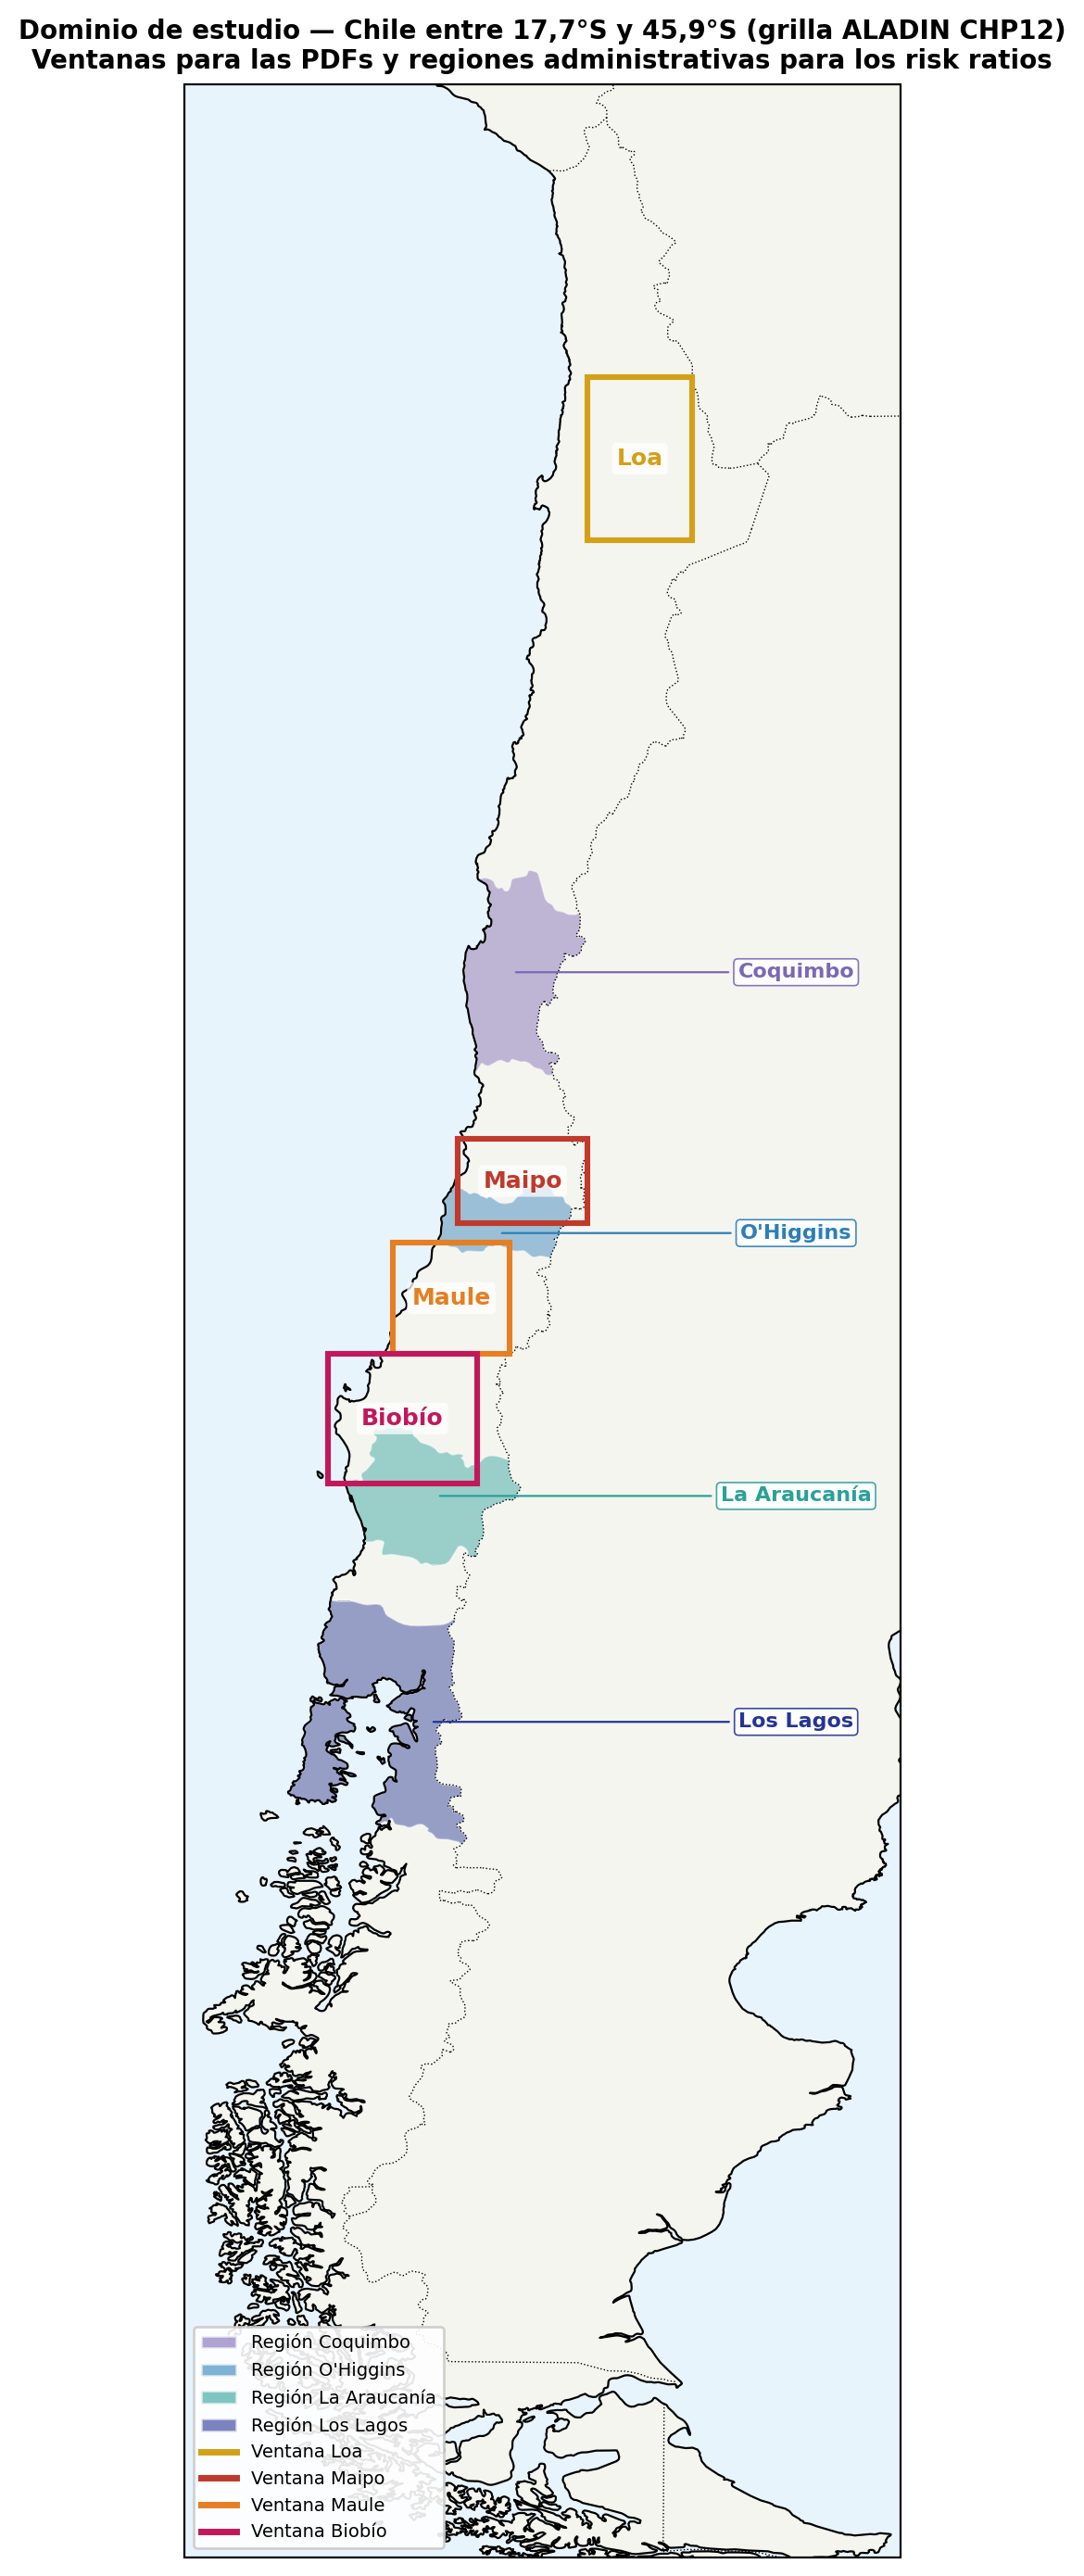
\includegraphics[width=1\linewidth,height=0.72\textheight,keepaspectratio,alt={Dominio de estudio sobre Chile continental. Los rectángulos indican las ventanas de latitud--longitud usadas para las PDFs de duración de dry spells: Loa (21,5--24,0°S; 68,2--69,8°O; 298 celdas), Maipo (33,2--34,5°S; 69,8--71,8°O; 154 celdas), Maule (34,8--36,5°S; 71,0--72,8°O; 171 celdas) y Biobío (36,5--38,5°S; 71,5--73,8°O; 243 celdas). Las ventanas aproximan las cuencas que les dan nombre sin coincidir con sus límites; en particular, la ventana Loa abarca la cuenca alta del Loa y la cuenca del Salar de Atacama, ambas representativas del norte árido. Las áreas sombreadas son las regiones administrativas usadas para los risk ratios: Coquimbo (239 celdas), O'Higgins (110), La Araucanía (223) y Los Lagos (324).}]{fig02_dominio_cuencas_regiones.png}
\caption[Dominio de estudio sobre Chile continental]{Dominio de estudio sobre Chile continental. Los rectángulos indican las ventanas de latitud--longitud usadas para las PDFs de duración de dry spells: Loa (21,5--24,0°S; 68,2--69,8°O; 298 celdas), Maipo (33,2--34,5°S; 69,8--71,8°O; 154 celdas), Maule (34,8--36,5°S; 71,0--72,8°O; 171 celdas) y Biobío (36,5--38,5°S; 71,5--73,8°O; 243 celdas). Las ventanas aproximan las cuencas que les dan nombre sin coincidir con sus límites; en particular, la ventana Loa abarca la cuenca alta del Loa y la cuenca del Salar de Atacama, ambas representativas del norte árido. Las áreas sombreadas son las regiones administrativas usadas para los risk ratios: Coquimbo (239 celdas), O'Higgins (110), La Araucanía (223) y Los Lagos (324).}\label{fig:dominio}
\end{figure}

\begin{longtable}[]{@{}
  >{\raggedright\arraybackslash}p{(\linewidth - 8\tabcolsep) * \real{0.2000}}
  >{\raggedright\arraybackslash}p{(\linewidth - 8\tabcolsep) * \real{0.2000}}
  >{\raggedright\arraybackslash}p{(\linewidth - 8\tabcolsep) * \real{0.2000}}
  >{\raggedright\arraybackslash}p{(\linewidth - 8\tabcolsep) * \real{0.2000}}
  >{\raggedright\arraybackslash}p{(\linewidth - 8\tabcolsep) * \real{0.2000}}@{}}
\caption{Conjuntos de datos: producto, rol, grilla, período y umbral de día húmedo.}\label{tab:datos}\tabularnewline
\toprule\noalign{}
\begin{minipage}[b]{\linewidth}\raggedright
Dataset
\end{minipage} & \begin{minipage}[b]{\linewidth}\raggedright
Rol
\end{minipage} & \begin{minipage}[b]{\linewidth}\raggedright
Grilla
\end{minipage} & \begin{minipage}[b]{\linewidth}\raggedright
Período
\end{minipage} & \begin{minipage}[b]{\linewidth}\raggedright
Umbral
\end{minipage} \\
\midrule\noalign{}
\endfirsthead
\toprule\noalign{}
\begin{minipage}[b]{\linewidth}\raggedright
Dataset
\end{minipage} & \begin{minipage}[b]{\linewidth}\raggedright
Rol
\end{minipage} & \begin{minipage}[b]{\linewidth}\raggedright
Grilla
\end{minipage} & \begin{minipage}[b]{\linewidth}\raggedright
Período
\end{minipage} & \begin{minipage}[b]{\linewidth}\raggedright
Umbral
\end{minipage} \\
\midrule\noalign{}
\endhead
\bottomrule\noalign{}
\endlastfoot
CR2MET v2.5 & Referencia observacional grillada & Lat/lon 0,05°; interpolada a ALADIN & 1980--2014 & R = 1 mm día$^{-1}$ \\
ALADIN CHP12 histórico & RCM CNRM-ALADIN64; forzado por CNRM-ESM2-1 & Nativa \textasciitilde12 km; 3 587 celdas en Chile & 1980--2014 (35 años) & R₀ = 5,285 mm día$^{-1}$ (criterio i) \\
ALADIN CHP12 SSP5-8.5 & Proyección del mismo RCM (análisis principal) & Idéntica al histórico & 2040--2074 (35 años) & Mismo R₀; RR con inicio mar--nov \\
ALADIN CHP12 SSP3-7.0 & Proyección del mismo RCM (sensibilidad de los risk ratios; S6) & Idéntica al histórico & 2040--2074 (35 años) & Mismo R₀ \\
\end{longtable}

\section{Definición de días húmedos/secos y dry spells}\label{sec:definicion}

Se define wet day (día húmedo) como un día con precipitación diaria pr ≥ R, donde R es un umbral en mm día$^{-1}$, y dry day (día seco) como un día con pr \textless{} R. Un dry spell es una racha consecutiva de dry days; su duración t es el número de días de la racha, con mínimo de un día (Figura~\ref{fig:esquema}). El umbral de 1 mm día$^{-1}$ en CR2MET sigue la convención ETCCDI/Climdex usada para CDD (Zhang et al., 2011; Sillmann et al., 2013a) y la misma definición operativa de dry day que Latoja et al.~(2025) y Herrera-Marín et al.~(2026). Dentro del dominio, ninguna de las series contiene días sin dato, por lo que todas las rachas se identifican sobre series diarias completas. En cada ventana temporal (1980--2014 o 2040--2074) se identifican todas las rachas de la serie diaria completa y se excluyen las censuradas, es decir, las que comienzan el primer día de la ventana o terminan el último, porque su duración verdadera es desconocida. Así, solo entran rachas cuyo inicio y término quedan dentro de la ventana. En Loa, donde las rachas pueden superar varios años, esta regla evita incluir duraciones truncadas, que subestimarían la cola, a costa de descartar algunas de las rachas más largas: las rachas censuradas representan menos del 1,1 \% del total en Loa y menos del 0,2 \% en las demás ventanas.

A diferencia del índice CDD, que resume cada año con su racha seca más larga, aquí se analizan todas las rachas, y una racha puede cruzar el 1 de enero: se conserva entera y se etiqueta con el año calendario de su inicio. En el norte árido esto es esencial, porque las rachas de cientos de días no caben en un año calendario. Para las PDFs y los mapas tampoco se restringe el análisis a una estación, a diferencia de Herrera-Marín et al.~(2026), quienes modelan inicios de racha en mayo--agosto; solo los risk ratios se limitan a rachas iniciadas entre marzo y noviembre (§\ref{sec:rr}). El objeto de estudio es la duración de cada racha, no el máximo anual ni la tasa de inicios.

\begin{figure}[htbp]
\centering
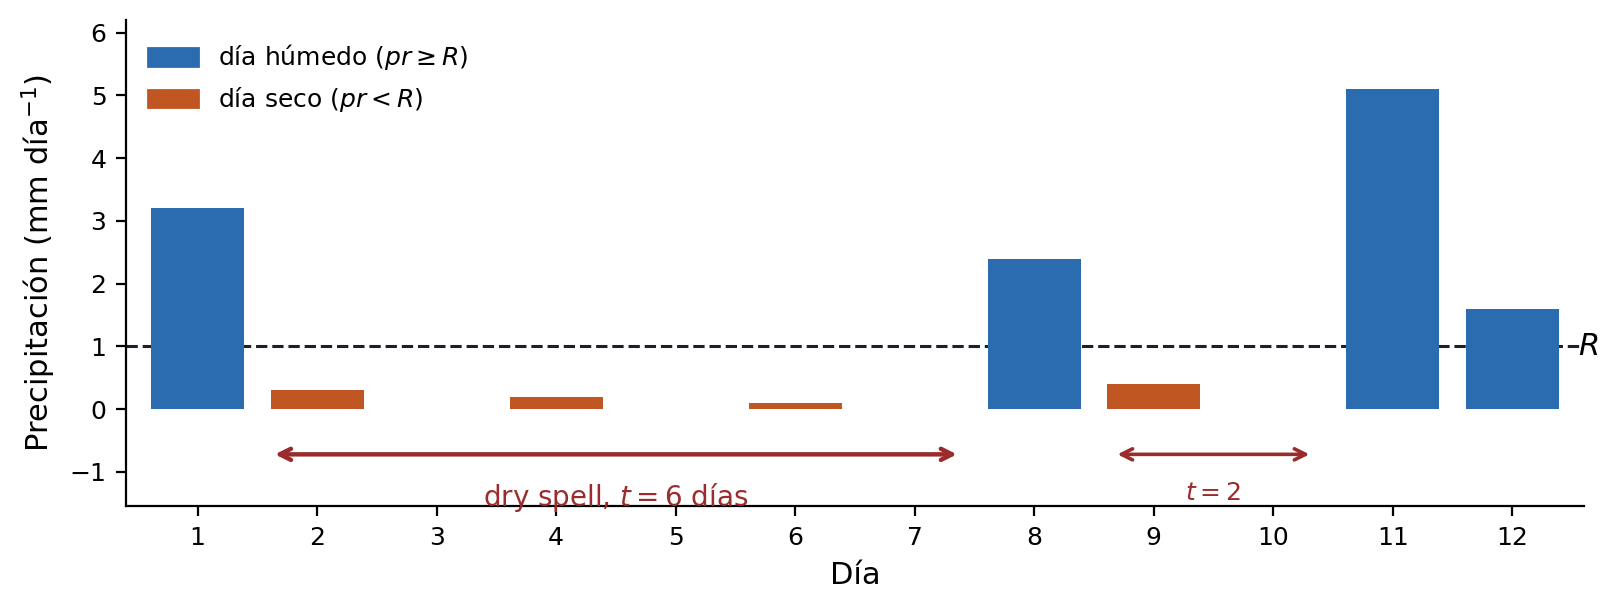
\includegraphics[width=1\linewidth,height=0.72\textheight,keepaspectratio,alt={Definición operativa. Un día es húmedo si pr ≥ R y seco si pr \textless{} R. Un dry spell es la racha consecutiva de días secos; su duración t es el número de días de la racha. En el ejemplo, R = 1 mm día$^{-1}$ produce un spell de t = 6 días y otro de t = 2 días, separados por un día húmedo. Los puntos marcan días secos con 0 mm.}]{fig_esquema_dryspell.png}
\caption[Definición operativa de día húmedo, día seco y dry spell]{Definición operativa. Un día es húmedo si pr ≥ R y seco si pr \textless{} R. Un dry spell es la racha consecutiva de días secos; su duración t es el número de días de la racha. En el ejemplo, R = 1 mm día$^{-1}$ produce un spell de t = 6 días y otro de t = 2 días, separados por un día húmedo. Los puntos marcan días secos con 0 mm.}\label{fig:esquema}
\end{figure}

La comparación histórica entre CR2MET y ALADIN requiere considerar sus diferencias en la frecuencia de días húmedos. Con R = 1 mm día$^{-1}$ en ambos productos, ALADIN presenta una fracción de días húmedos sustancialmente mayor que CR2MET (§\ref{sec:calibracion}), coherente con el sesgo de llovizna de los modelos (Stephens et al., 2010; Petrova et al., 2024; Martinez-Villalobos et al., 2022). Ese exceso fragmenta las rachas secas y produce spells artificialmente más cortos y numerosos, de modo que un umbral común de 1 mm no permite una comparación equitativa de la persistencia seca.

Por ello el análisis principal adopta el criterio i (umbral global calibrado): CR2MET con R = 1 mm día$^{-1}$ y ALADIN con R₀ = 5,285 mm día$^{-1}$, elegido para igualar la fracción espacial media de wet days de CR2MET a 1 mm (§\ref{sec:calibracion}). Este umbral dependiente del modelo sigue el criterio usado para evaluar PDFs de duración de dry spells frente a observaciones (Leung et al., 2022, sec.~3.b). Como sensibilidad se consideran el criterio ii (1 mm día$^{-1}$ en ambos) y el criterio iii (calibración local: un R₀(x,y) por píxel, de modo que en cada celda la fracción temporal de wet days de ALADIN iguale la de CR2MET a 1 mm). El criterio i es la configuración de los resultados principales; ii y iii permiten separar cuánto del sesgo histórico se debe a la definición de día húmedo y cuánto permanece como diferencia estructural del modelo (Tabla~\ref{tab:criterios}).

\begin{longtable}[]{@{}
  >{\raggedright\arraybackslash}p{(\linewidth - 6\tabcolsep) * \real{0.2500}}
  >{\raggedright\arraybackslash}p{(\linewidth - 6\tabcolsep) * \real{0.2500}}
  >{\raggedright\arraybackslash}p{(\linewidth - 6\tabcolsep) * \real{0.2500}}
  >{\raggedright\arraybackslash}p{(\linewidth - 6\tabcolsep) * \real{0.2500}}@{}}
\caption[Criterios de umbral para definir días húmedos]{Criterios de umbral para definir días húmedos. El análisis principal usa el criterio i.}\label{tab:criterios}\tabularnewline
\toprule\noalign{}
\begin{minipage}[b]{\linewidth}\raggedright
Criterio
\end{minipage} & \begin{minipage}[b]{\linewidth}\raggedright
CR2MET
\end{minipage} & \begin{minipage}[b]{\linewidth}\raggedright
ALADIN
\end{minipage} & \begin{minipage}[b]{\linewidth}\raggedright
Uso
\end{minipage} \\
\midrule\noalign{}
\endfirsthead
\toprule\noalign{}
\begin{minipage}[b]{\linewidth}\raggedright
Criterio
\end{minipage} & \begin{minipage}[b]{\linewidth}\raggedright
CR2MET
\end{minipage} & \begin{minipage}[b]{\linewidth}\raggedright
ALADIN
\end{minipage} & \begin{minipage}[b]{\linewidth}\raggedright
Uso
\end{minipage} \\
\midrule\noalign{}
\endhead
\bottomrule\noalign{}
\endlastfoot
i (global) & 1 mm & R₀ = 5,285 mm (único, Chile) & Resultados principales \\
ii (mismo umbral) & 1 mm & 1 mm & Sensibilidad: sesgo sin calibrar \\
iii (local) & 1 mm & R₀(x,y) por píxel & Sensibilidad espacial \\
\end{longtable}

\section{Calibración del umbral R₀}\label{sec:calibracion}

La calibración de R₀ busca el umbral tal que el promedio espacial sobre Chile continental de la fracción temporal de días con pr ≥ R en ALADIN iguale la fracción correspondiente de CR2MET con R = 1 mm día$^{-1}$. Si F(R) denota esa fracción espacial media de wet days, calculada con igual peso para cada celda de la grilla de ALADIN, se resuelve F\_ALADIN(R₀) = F\_CR2MET(1 mm) mediante bisección. En 1980--2014, CR2MET a 1 mm produce F = 20,94 \% y ALADIN a 1 mm produce F = 30,68 \% (+9,7 puntos porcentuales). El umbral R₀ = 5,285 mm día$^{-1}$ reproduce F = 20,94 \% en ALADIN (Figura~\ref{fig:calibracion}).

\begin{figure}[htbp]
\centering
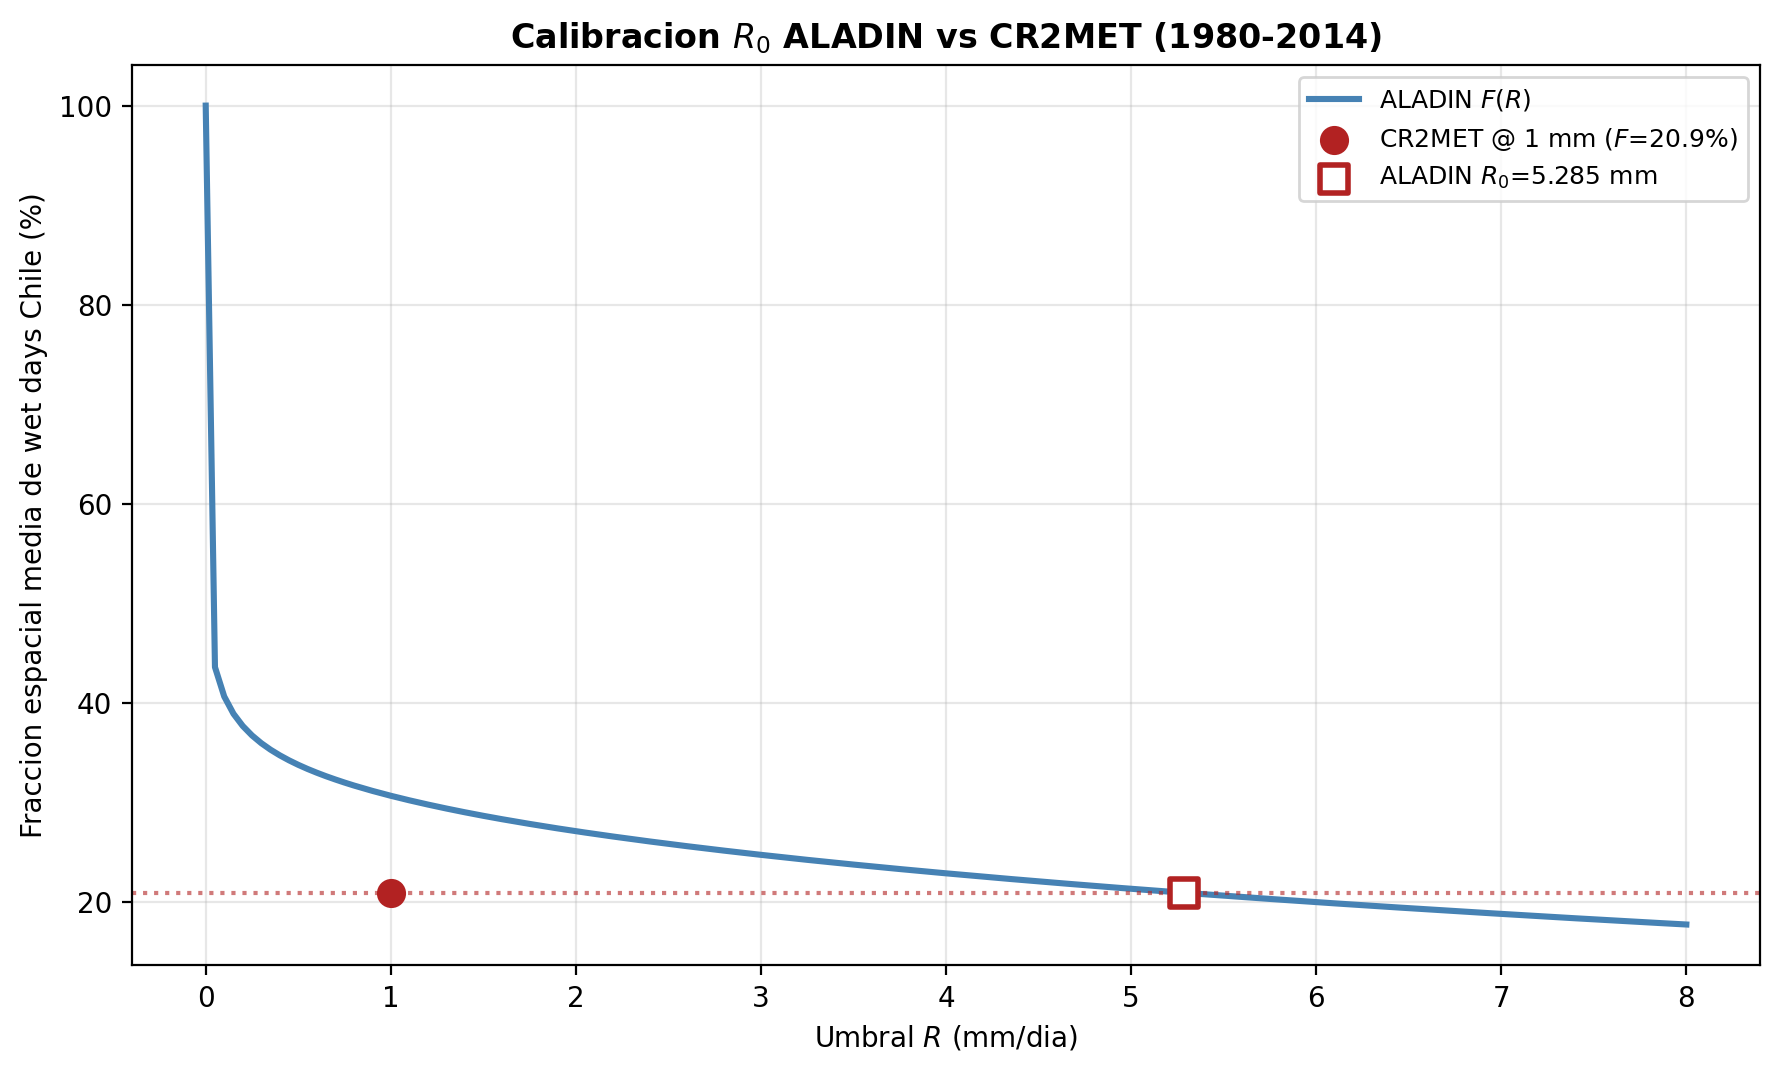
\includegraphics[width=1\linewidth,height=0.72\textheight,keepaspectratio,alt={Calibración del umbral de día húmedo en ALADIN frente a CR2MET (1980--2014). La curva azul es F(R), la fracción media de días húmedos de ALADIN en Chile continental en función del umbral R. El punto azul es ALADIN a 1 mm (F = 30,7 \%) y el punto rojo es CR2MET a 1 mm (F = 20,9 \%); la flecha indica el exceso de días húmedos de ALADIN (+9,7 puntos porcentuales), que, sin calibrar, acorta las rachas secas. El cuadrado marca R₀ = 5,285 mm día$^{-1}$, umbral con el que ALADIN iguala la fracción de CR2MET.}]{fig03_calibracion_R0_ftau.png}
\caption[Calibración del umbral de día húmedo en ALADIN frente a CR2MET (1980--2014)]{Calibración del umbral de día húmedo en ALADIN frente a CR2MET (1980--2014). La curva azul es F(R), la fracción media de días húmedos de ALADIN en Chile continental en función del umbral R. El punto azul es ALADIN a 1 mm (F = 30,7 \%) y el punto rojo es CR2MET a 1 mm (F = 20,9 \%); la flecha indica el exceso de días húmedos de ALADIN (+9,7 puntos porcentuales), que, sin calibrar, acorta las rachas secas. El cuadrado marca R₀ = 5,285 mm día$^{-1}$, umbral con el que ALADIN iguala la fracción de CR2MET.}\label{fig:calibracion}
\end{figure}

R₀ representa un umbral que hace equivalentes las frecuencias de días húmedos de ambos productos: un día de ALADIN con 3 mm se trata como seco porque, en frecuencia, corresponde a un día bajo 1 mm en CR2MET. La calibración iguala la frecuencia en promedio sobre Chile, no en cada celda; el criterio iii (§\ref{sec:definicion}) evalúa ese efecto calibrando un umbral por píxel. Igualar la frecuencia de días húmedos tampoco impone que se distribuyan igual en el tiempo: dos series con el mismo número de días húmedos pueden producir rachas secas muy distintas si esos días aparecen agrupados o dispersos. Por ello, las diferencias de duración que persisten tras la calibración reflejan la organización temporal de la precipitación en el modelo y no solo su exceso de días húmedos.

\section{Construcción y normalización de las PDFs}\label{sec:pdfs}

Para caracterizar la distribución de duraciones se construyen PDFs empíricas de la variable t (días), con bins uniformes en log₁₀(t), siguiendo la convención de PDFs de precipitación diaria (Martinez-Villalobos y Neelin, 2018; Martinez-Villalobos et al., 2022). En cada cuenca se usan los mismos bins para CR2MET, ALADIN histórico y ALADIN futuro: se generan 26 bordes en escala logarítmica entre 1 día y la duración máxima observada entre los tres conjuntos, y se redondean a enteros. Como las duraciones son enteras, los bordes repetidos se fusionan, de modo que cada bin contiene un número entero de días y el número efectivo de bins es de 21 a 23 según la cuenca.

En cada bin, f(t) es el número de spells en el intervalo dividido por el ancho de bin, de modo que el área bajo la curva es igual al número total de spells del pool y los cambios en frecuencias y en forma son visibles a la vez. El binning solo afecta la representación gráfica: los estadísticos de la Tabla~\ref{tab:estadisticos} y los risk ratios se calculan directamente sobre las duraciones.

\section{Agrupación regional y estadísticas espaciales}\label{sec:pool}

Para las PDFs por cuenca se adopta un pool regional: todos los dry spells de todos los píxeles de la ventana se agrupan en un único conjunto de eventos (Martinez-Villalobos y Neelin, 2018). El pool aumenta el tamaño muestral y permite resolver la cola; a cambio, mezcla heterogeneidad espacial dentro de la caja. Como los píxeles vecinos no son independientes, n\_spells no debe leerse como tamaño muestral efectivo para inferencia estadística.

Para los mapas se calculan, en cada píxel, la duración media y el percentil 99 de las duraciones (t99), y se reportan las diferencias Δ = ALADIN − CR2MET en 1980--2014. Los estadísticos solo se calculan en píxeles con al menos 30 spells en el período. La significancia de Δ se evalúa con bootstrap por años (1 000 réplicas). Primero se identifican los spells en la serie diaria de cada píxel con las reglas de §\ref{sec:definicion}, incluida la exclusión de rachas censuradas en los bordes del período. Cada spell conserva su duración íntegra aunque cruce el 1 de enero y se asigna al año calendario de su inicio. Con ello se forma, por píxel y producto, un conjunto \{año: vector de duraciones\}.

En cada réplica se sortean 35 años calendario con reemplazo, usando el mismo sorteo para CR2MET y ALADIN (bootstrap pareado). Se concatenan las duraciones de todos los spells cuyo año de inicio figura en el sorteo y se recalculan la media o t99 de cada producto y su diferencia Δ\emph{. El intervalo de confianza al 95 \% de Δ corresponde a los percentiles 2,5 y 97,5 de las 1 000 réplicas de Δ}, y Δ se considera significativo cuando el intervalo no incluye el cero.

Como se evalúan unas 3 500 celdas con α = 5 \%, cabe esperar que alrededor del 5 \% resulte significativo por azar; los porcentajes de celdas significativas se interpretan en relación con esa referencia.

\section{Risk ratios y cambios futuros}\label{sec:rr}

El cambio proyectado en la ocurrencia de dry spells largos se cuantifica con el risk ratio

\emph{(1) RR(D) = N\_fut(t ≥ D) / N\_hist(t ≥ D)}

donde N(t ≥ D) es el número de dry spells con duración de al menos D días en ALADIN futuro (2040--2074) e histórico (1980--2014), ambos con R₀ = 5,285 mm día$^{-1}$ y con las reglas de §\ref{sec:definicion}, incluida la exclusión de rachas censuradas. Como ambos períodos tienen la misma longitud (35 años), RR(D) es también una razón de frecuencias; RR(D) \textgreater{} 1 indica más rachas largas en el futuro. Al no normalizar por el número total de spells de cada período, RR(D) es consistente con las PDFs (§\ref{sec:pdfs}) y refleja el cambio en la ocurrencia de eventos largos, no solo en su fracción relativa.

Los risk ratios se calculan sobre pools de las cuatro regiones administrativas (§\ref{sec:datos}), considerando solo spells cuyo día de inicio cae entre marzo y noviembre (otoño, invierno y primavera), meses que concentran entre el 85 \% y el 97 \% de la precipitación anual en esas regiones. En verano la precipitación es escasa, sobre todo en Chile central, y las rachas largas forman parte del ciclo estacional esperado; los spells que comienzan en noviembre se cuentan con su duración completa aunque se extiendan al verano. Las PDFs, en cambio, incluyen spells de todo el año. Se calculan curvas RR(D) para D entre 5 y 60 días, y D = 20 días se usa como valor de referencia porque corresponde aproximadamente al percentil 90 de las duraciones en Chile central (Tabla~\ref{tab:estadisticos}). Los intervalos de confianza al 95 \% se obtienen con bootstrap por años (1 000 réplicas): en cada réplica se sortean con reemplazo 35 años de inicio del histórico y, de forma independiente, 35 del futuro, y se recalcula el cociente de conteos. Como se remuestrean años completos para todos los píxeles de la región a la vez, el procedimiento conserva la correlación espacial entre píxeles. El cambio se considera significativo cuando el IC95 queda por completo por encima de 1 (aumento) o por debajo de 1 (disminución). Como la curva evalúa varios valores de D, se interpreta su comportamiento conjunto y no un umbral aislado.

\section{Sensibilidad a la elección del umbral}\label{sec:sensibilidad}

Para evaluar cuánto dependen los resultados de la definición de día húmedo, la comparación histórica entre CR2MET y ALADIN se repite con los tres criterios de la Tabla~\ref{tab:criterios}. A escala de Chile continental, se recalculan los mapas de duración media y t99, sus diferencias Δ y su significancia con el procedimiento de §\ref{sec:pool}. A escala de cuenca, se comparan las PDFs de Loa, Maipo, Maule y Biobío en 1980--2014 para CR2MET a 1 mm y para ALADIN a 1 mm, a R₀ global y a R₀ local, con los bins de §\ref{sec:pdfs}. Además, los risk ratios de §\ref{sec:rr} se recalculan con 1 mm en ALADIN para comprobar que la señal futura no depende de la calibración. Los resultados de estas pruebas (Tablas~\ref{tab:S1}--\ref{tab:S3}, Figuras~\ref{fig:S1} y~\ref{fig:S3}) y el mapa de R₀ local (Figura~\ref{fig:S2}) se presentan en el material suplementario.

\section{Herramientas computacionales y reproducibilidad}\label{sec:software}

\pendiente{describir el software (Python, xarray, numpy, cartopy) y remitir al
Anexo B con los scripts que generan cada figura y tabla.}

\pendiente{agregar un diagrama de flujo de la metodología: datos → regrillado →
definición de rachas → calibración de R₀ → PDFs, mapas y bootstrap →
risk ratios → sensibilidades.}

\chapter{Evaluación histórica (1980–2014)}\label{cap:4}

\section{Evaluación histórica (1980--2014)}\label{sec:eval}

Esta sección responde la primera pregunta del estudio: una vez igualada la frecuencia de días húmedos (criterio i; R₀ = 5,285 mm día$^{-1}$ en ALADIN y R = 1 mm día$^{-1}$ en CR2MET), ¿reproduce ALADIN la distribución histórica de duraciones de dry spells?

\subsection{Climatología de persistencia en CR2MET}\label{sec:climatologia}

CR2MET muestra un contraste norte--sur marcado en la persistencia de rachas secas, coherente con el gradiente climático de Chile y con diagnósticos recientes de dry spells en la zona central (Latoja et al., 2025; Herrera-Marín et al., 2026). En el norte árido la duración media supera con creces el mes: en la ventana del Loa el pool regional tiene media de 65,6 días y p99 de 456 días, con máximos por encima de 1 400 días. En el sur más húmedo las rachas son cortas y numerosas: en Biobío la media es 6,2 días y el p99, 44 días. Maipo y Maule ocupan el tramo intermedio (medias de 11,0 y 9,5 días; p99 de 119 y 83 días). Ese gradiente no es un artefacto de un índice anual: aparece tanto en la media como en la cola (t99) a escala de píxel (Figura~\ref{fig:mapas}, columnas CR2MET).

Dos implicaciones siguen de inmediato. Primera: un mismo estadístico agregado ---por ejemplo, el CDD--- comprime climas distintos en un solo máximo por año (Zhang et al., 2011; Sillmann et al., 2013a), mientras que aquí la cola de Loa y la de Biobío no son conmensurables. Segunda: cualquier evaluación de ALADIN tiene que respetar ese contraste latitudinal; un sesgo aceptable en el sur húmedo puede ser grave en el desierto si se pierde la cola de spells de cientos de días.

\subsection{ALADIN reproduce el gradiente espacial, pero subestima la persistencia y la cola}\label{sec:sesgo}

Con el criterio i, ALADIN reproduce el patrón espacial ---norte persistente, sur de rachas cortas--- pero subestima la duración. Sobre Chile continental, la duración media espacial es 42,1 días en CR2MET y 34,0 días en ALADIN (Δ, media espacial de las diferencias por píxel, = −8,2 días). El sesgo es mayor en la cola: t99 espacial de 221,1 días frente a 175,3 días (Δ = −46,3 días). Los mapas de diferencia (Figura~\ref{fig:mapas}) muestran Δ negativo de manera generalizada, más intenso en la transición norte--centro, donde CR2MET resuelve spells extremadamente largos que ALADIN acorta. ALADIN es significativamente más corto en cerca de dos tercios de los píxeles para la duración media (65 \%) y en el 43 \% para t99 (bootstrap por años, IC95 de Δ que no incluye cero).

Ese residuo no se explica solo por el umbral. Con 1 mm en ambos productos (criterio ii) el sesgo aumenta mucho (Δ media ≈ −27 días; Δ t99 ≈ −135 días). El R₀ global (criterio i) lo reduce sustancialmente; a escala nacional, el R₀ local lo reduce algo más, pero no elimina el sesgo de cola (Tabla~\ref{tab:S1}; Figura~\ref{fig:S1}). El análisis principal usa el criterio i porque corrige la definición de día húmedo sin un campo heterogéneo de umbrales; el sesgo residual se interpreta como limitación del RCM.

\begin{figure}[htbp]
\centering
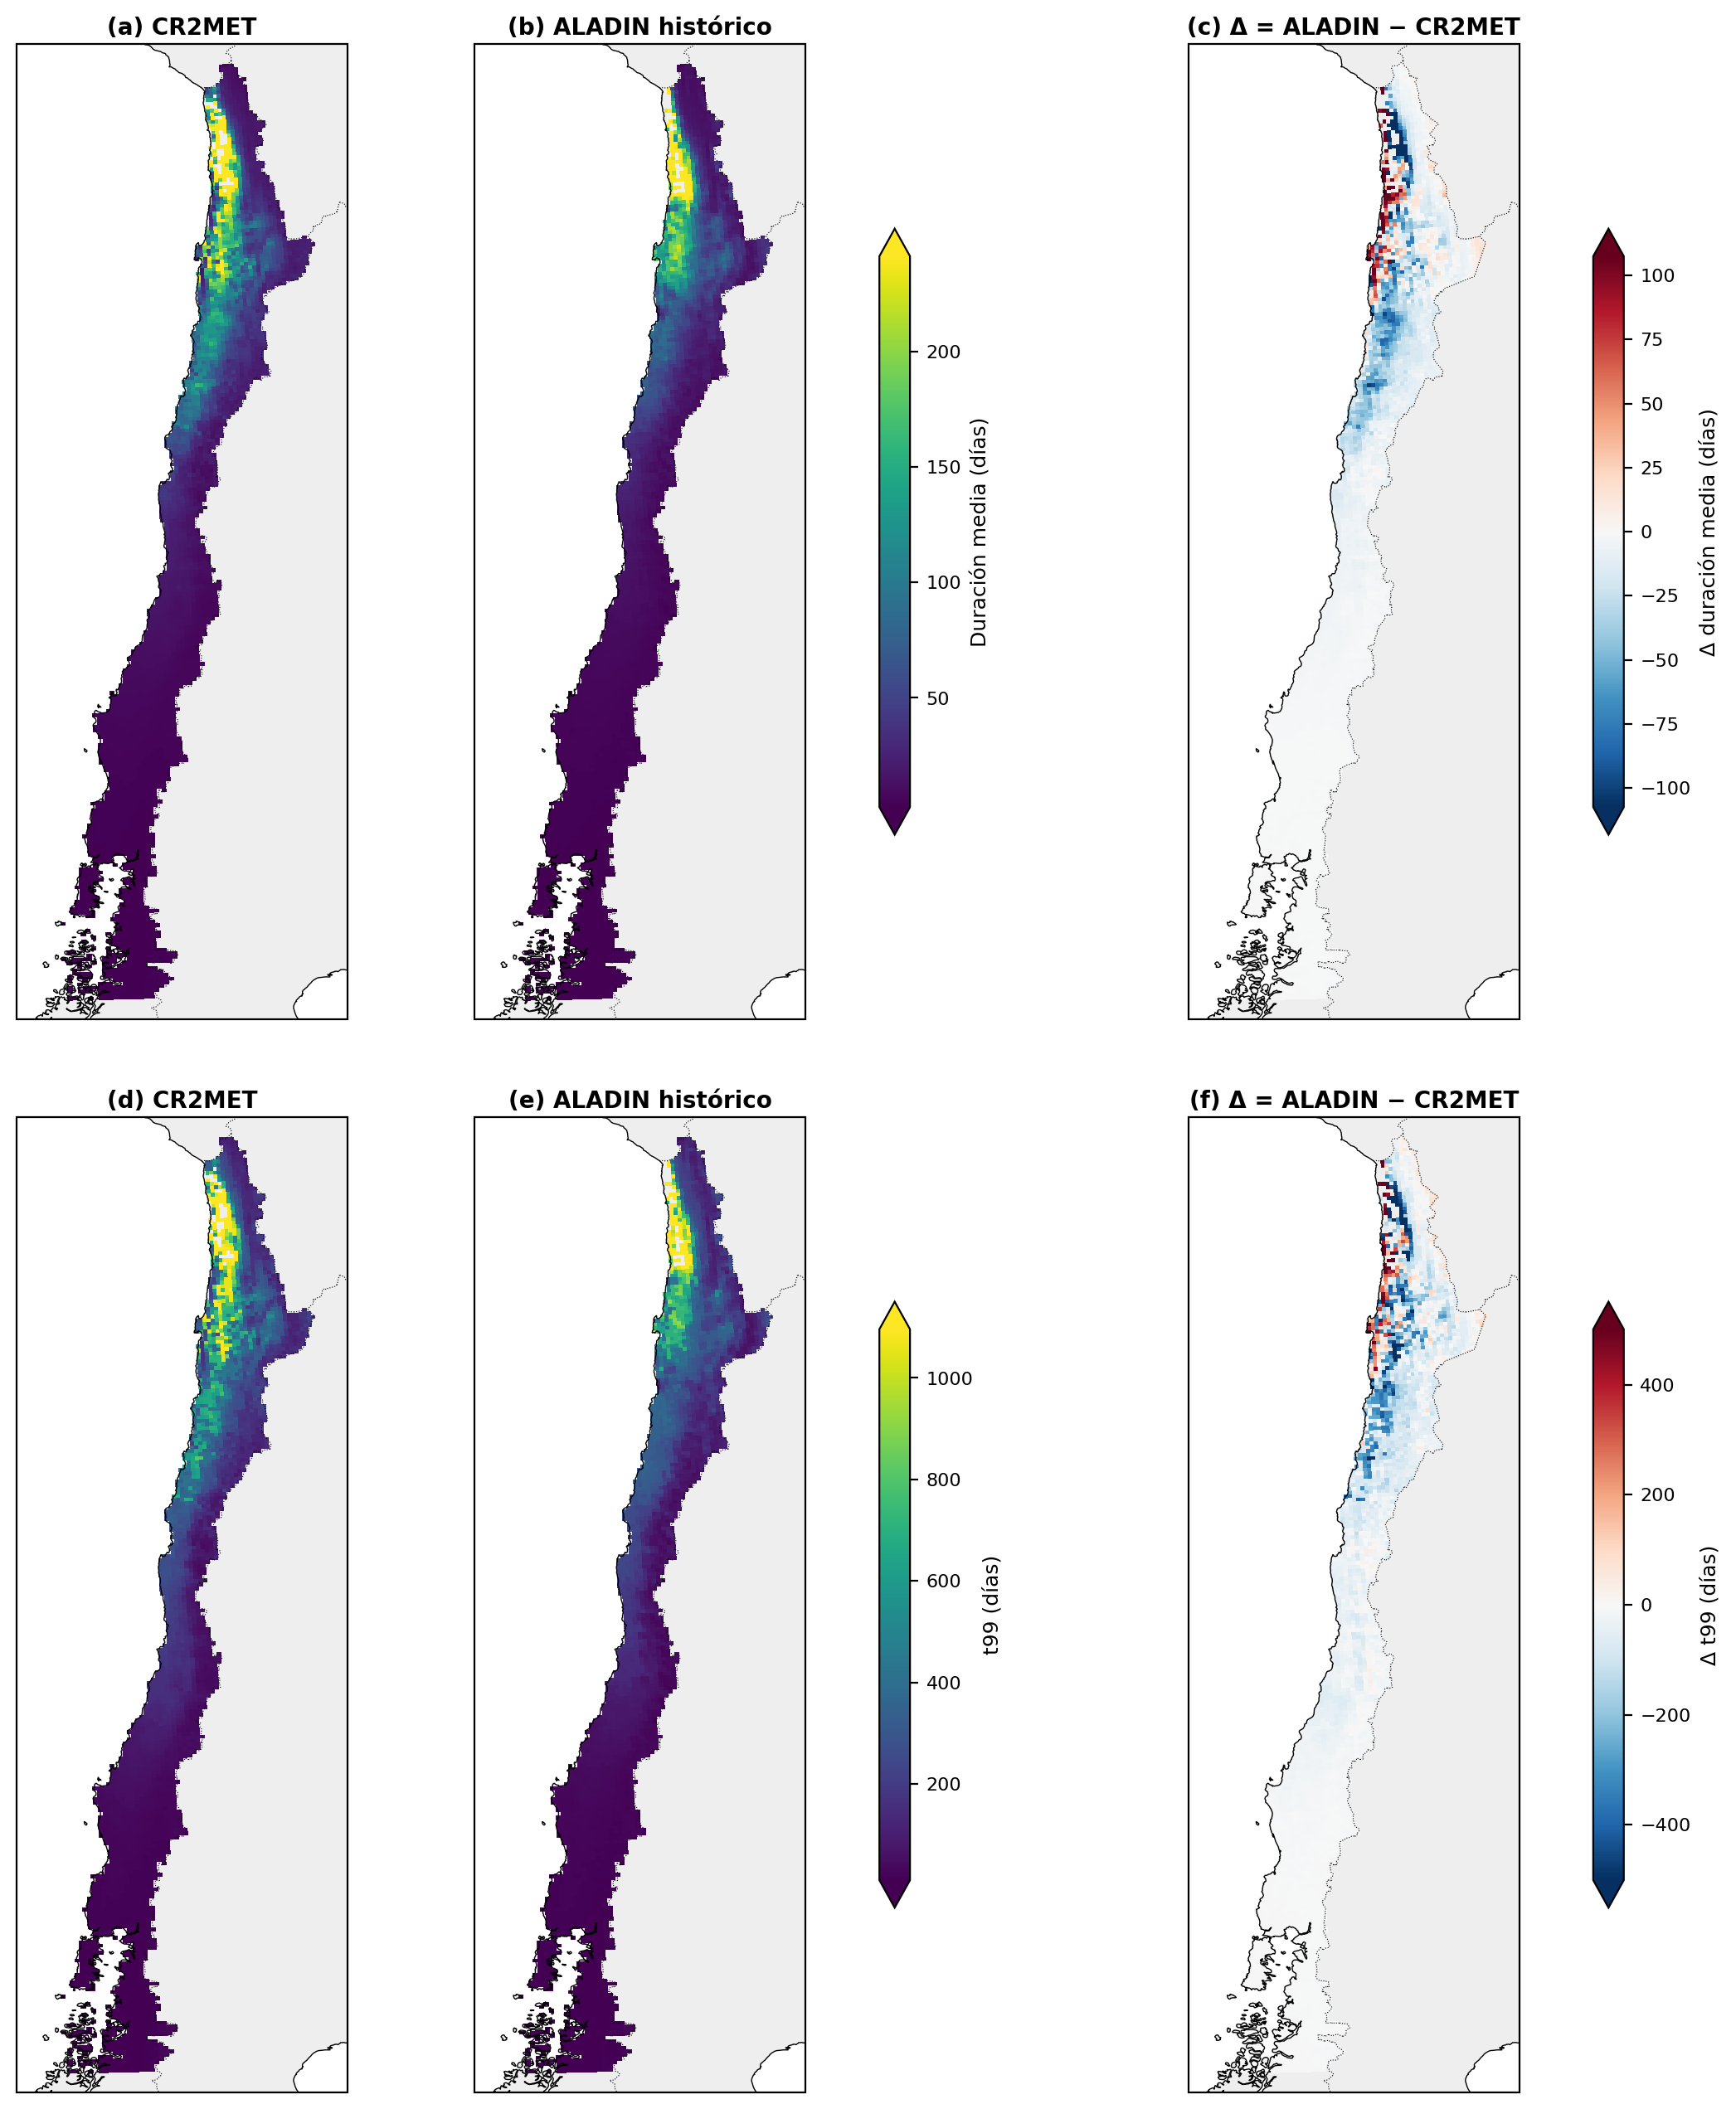
\includegraphics[width=1\linewidth,height=0.72\textheight,keepaspectratio,alt={Persistencia histórica de dry spells (1980--2014), criterio i. Fila superior: duración media (días). Fila inferior: percentil 99 de las duraciones, t99 (días). Columnas: CR2MET regrillado (R = 1 mm), ALADIN histórico (R₀ = 5,285 mm) y Δ = ALADIN − CR2MET. Ambas fuentes reproducen el gradiente norte--sur; ALADIN subestima media y cola, con Δ negativo más marcado en t99.}]{fig32_persistencia_spatial_only.png}
\caption[Persistencia histórica de dry spells (1980--2014), criterio i]{Persistencia histórica de dry spells (1980--2014), criterio i. Fila superior: duración media (días). Fila inferior: percentil 99 de las duraciones, t99 (días). Columnas: CR2MET regrillado (R = 1 mm), ALADIN histórico (R₀ = 5,285 mm) y Δ = ALADIN − CR2MET. Ambas fuentes reproducen el gradiente norte--sur; ALADIN subestima media y cola, con Δ negativo más marcado en t99.}\label{fig:mapas}
\end{figure}

\subsection{PDFs regionales: buen acuerdo en el centro-sur y mayor sesgo de cola en el norte}\label{sec:pdfs_hist}

Las distribuciones regionales confirman que el acuerdo entre CR2MET y ALADIN es mayor en el centro-sur y que el principal desacuerdo se concentra en la cola del norte árido (Figura~\ref{fig:pdfs}; Tabla~\ref{tab:estadisticos}). En Maipo, Maule y Biobío, CR2MET e histórico de ALADIN son aproximadamente paralelos: ALADIN captura la forma y subestima de manera moderada las duraciones (medias 8,6 frente a 11,0 días en Maipo; 7,3 frente a 9,5 en Maule; 5,3 frente a 6,2 en Biobío). En Loa el desacuerdo se concentra en la cola: CR2MET mantiene más probabilidad en spells de cientos de días (p99 = 456 días frente a 360 días en ALADIN; máximo 1 419 frente a 1 156). ALADIN produce, en todas las cuencas, más spells que CR2MET (p.~ej. 66 267 frente a 55 015 en Loa), coherente con rachas algo más cortas aunque la frecuencia de wet days ya está emparejada.

En conjunto, la evaluación histórica muestra que ALADIN reproduce mejor la forma de la distribución en Maipo, Maule y Biobío, mientras que subestima las duraciones en el norte árido y en la cola extrema.

\begin{longtable}[]{@{}llllllll@{}}
\caption[Estadísticos del pool regional de duraciones de dry spells (criterio i; 1980--2014 y 2040--2074)]{Estadísticos del pool regional de duraciones de dry spells (criterio i; 1980--2014 y 2040--2074). n\_spells es el número de rachas en el pool; p90 y p99 están en días.}\label{tab:estadisticos}\tabularnewline
\toprule\noalign{}
Cuenca & Producto & n\_spells & Media & Mediana & p90 & p99 & Máx. \\
\midrule\noalign{}
\endfirsthead
\toprule\noalign{}
Cuenca & Producto & n\_spells & Media & Mediana & p90 & p99 & Máx. \\
\midrule\noalign{}
\endhead
\bottomrule\noalign{}
\endlastfoot
Loa & CR2MET hist & 55 015 & 65,6 & 23 & 185 & 456 & 1 419 \\
Loa & ALADIN hist & 66 267 & 54,6 & 22 & 143 & 360 & 1 156 \\
Loa & ALADIN fut & 64 043 & 56,6 & 25 & 151 & 385 & 1 853 \\
Maipo & CR2MET hist & 150 209 & 11,0 & 5 & 23 & 119 & 283 \\
Maipo & ALADIN hist & 181 049 & 8,6 & 4 & 18 & 87 & 194 \\
Maipo & ALADIN fut & 159 887 & 10,0 & 4 & 21 & 112 & 224 \\
Maule & CR2MET hist & 184 462 & 9,5 & 5 & 21 & 83 & 206 \\
Maule & ALADIN hist & 228 077 & 7,3 & 4 & 17 & 57 & 160 \\
Maule & ALADIN fut & 202 463 & 8,6 & 4 & 19 & 76 & 188 \\
Biobío & CR2MET hist & 344 251 & 6,2 & 4 & 14 & 44 & 109 \\
Biobío & ALADIN hist & 399 130 & 5,3 & 3 & 12 & 34 & 153 \\
Biobío & ALADIN fut & 370 260 & 6,0 & 3 & 14 & 39 & 120 \\
\end{longtable}

\begin{figure}[htbp]
\centering
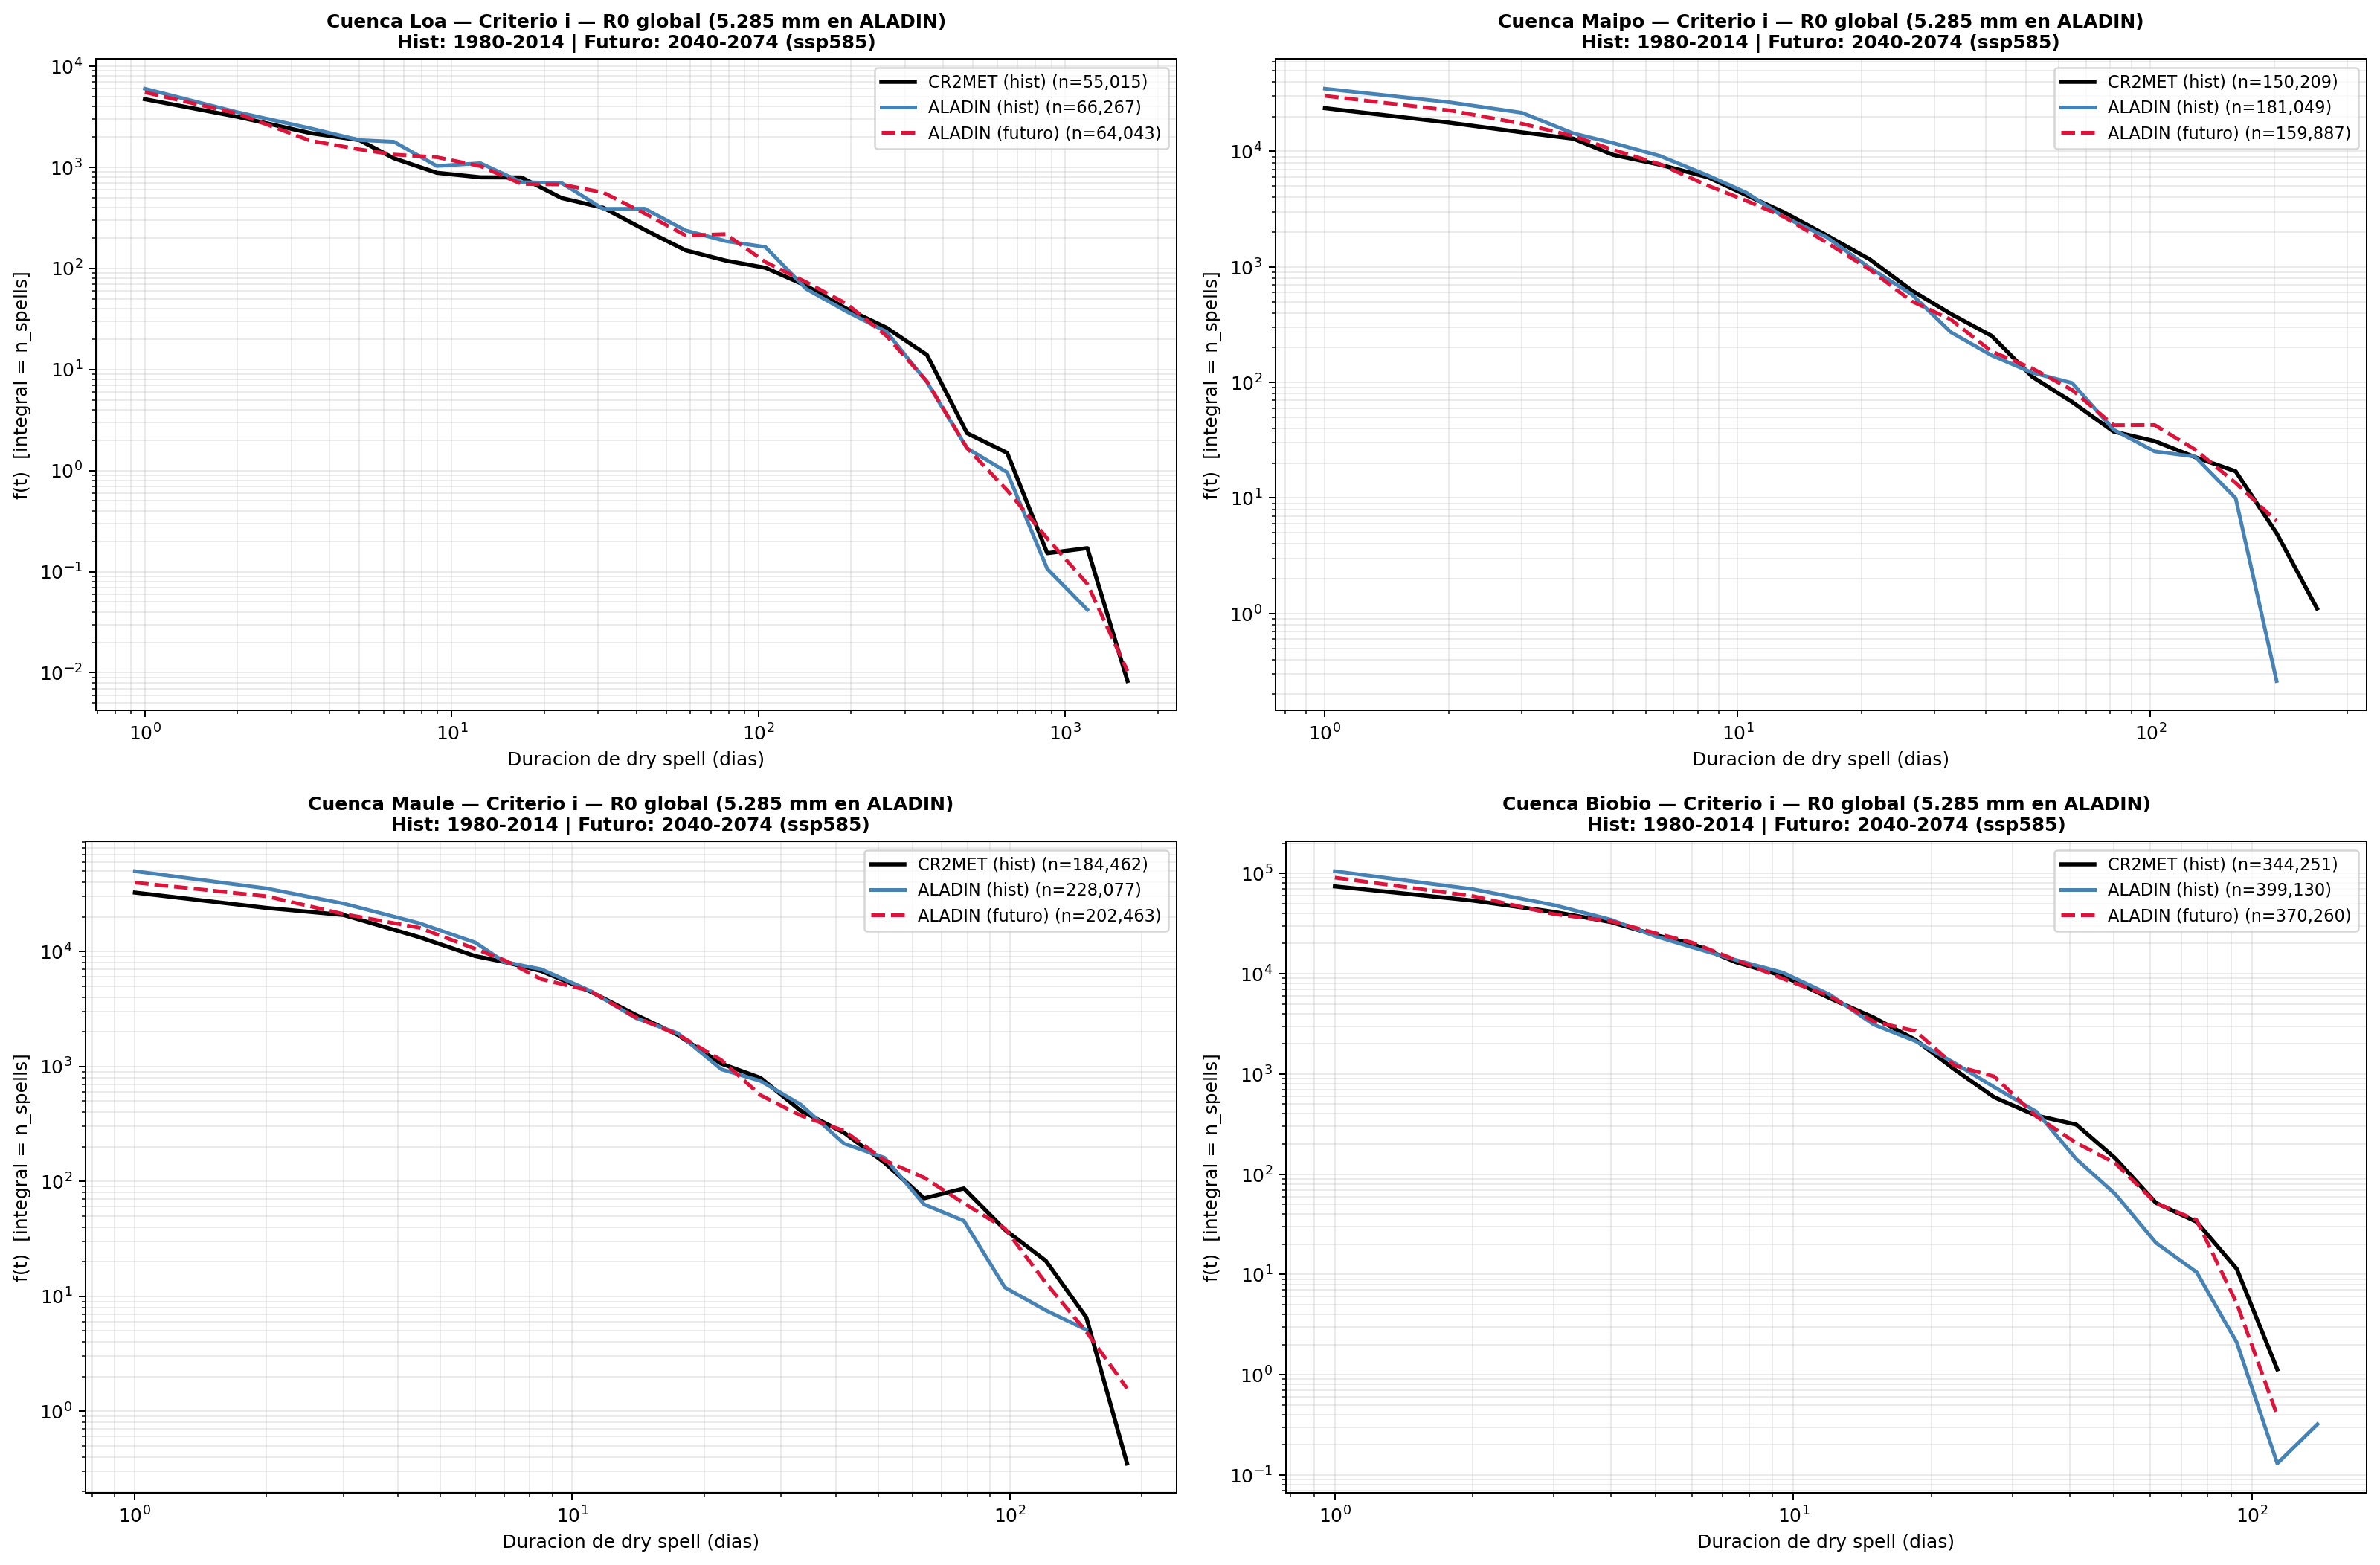
\includegraphics[width=1\linewidth,height=0.72\textheight,keepaspectratio,alt={PDFs empíricas de duración de dry spells (criterio i, escala log--log; ∫ f dt = n\_spells). Negro: CR2MET 1980--2014. Azul: ALADIN histórico. Rojo discontinuo: ALADIN futuro (SSP5-8.5, 2040--2074). El histórico de ALADIN sigue la forma de CR2MET en Maipo, Maule y Biobío, y pierde cola en Loa. El futuro se discute en §\ref{sec:pdfs_fut}: n\_spells disminuye y la cola derecha se extiende en las cuencas centrales y en Biobío.}]{fig42_pdf_cuencas_loglog_panel.png}
\caption[PDFs empíricas de duración de dry spells (criterio i, escala log--log; ∫ f dt = n\_spells)]{PDFs empíricas de duración de dry spells (criterio i, escala log--log; ∫ f dt = n\_spells). Negro: CR2MET 1980--2014. Azul: ALADIN histórico. Rojo discontinuo: ALADIN futuro (SSP5-8.5, 2040--2074). El histórico de ALADIN sigue la forma de CR2MET en Maipo, Maule y Biobío, y pierde cola en Loa. El futuro se discute en §\ref{sec:pdfs_fut}: n\_spells disminuye y la cola derecha se extiende en las cuencas centrales y en Biobío.}\label{fig:pdfs}
\end{figure}

\pendiente{decidir si las sensibilidades S1--S3 y S5 (Anexo A) se integran aquí
como sección de robustez.}

\chapter{Proyecciones futuras (SSP5-8.5, 2040–2074)}\label{cap:5}

La segunda pregunta es si, bajo SSP5-8.5, cambia la probabilidad de rachas prolongadas ---no solo el acumulado anual. La comparación es ALADIN histórico versus ALADIN futuro, con el mismo R₀. A escala de Chile, el modelo proyecta menos precipitación anual en el centro-sur (del orden de −10 a −20 \% en gran parte del dominio) y, a la vez, un aumento de la duración media de dry spells de varios días en el norte y el centro (Figura~\ref{fig:mapas_futuro}).

\begin{figure}[htbp]
\centering
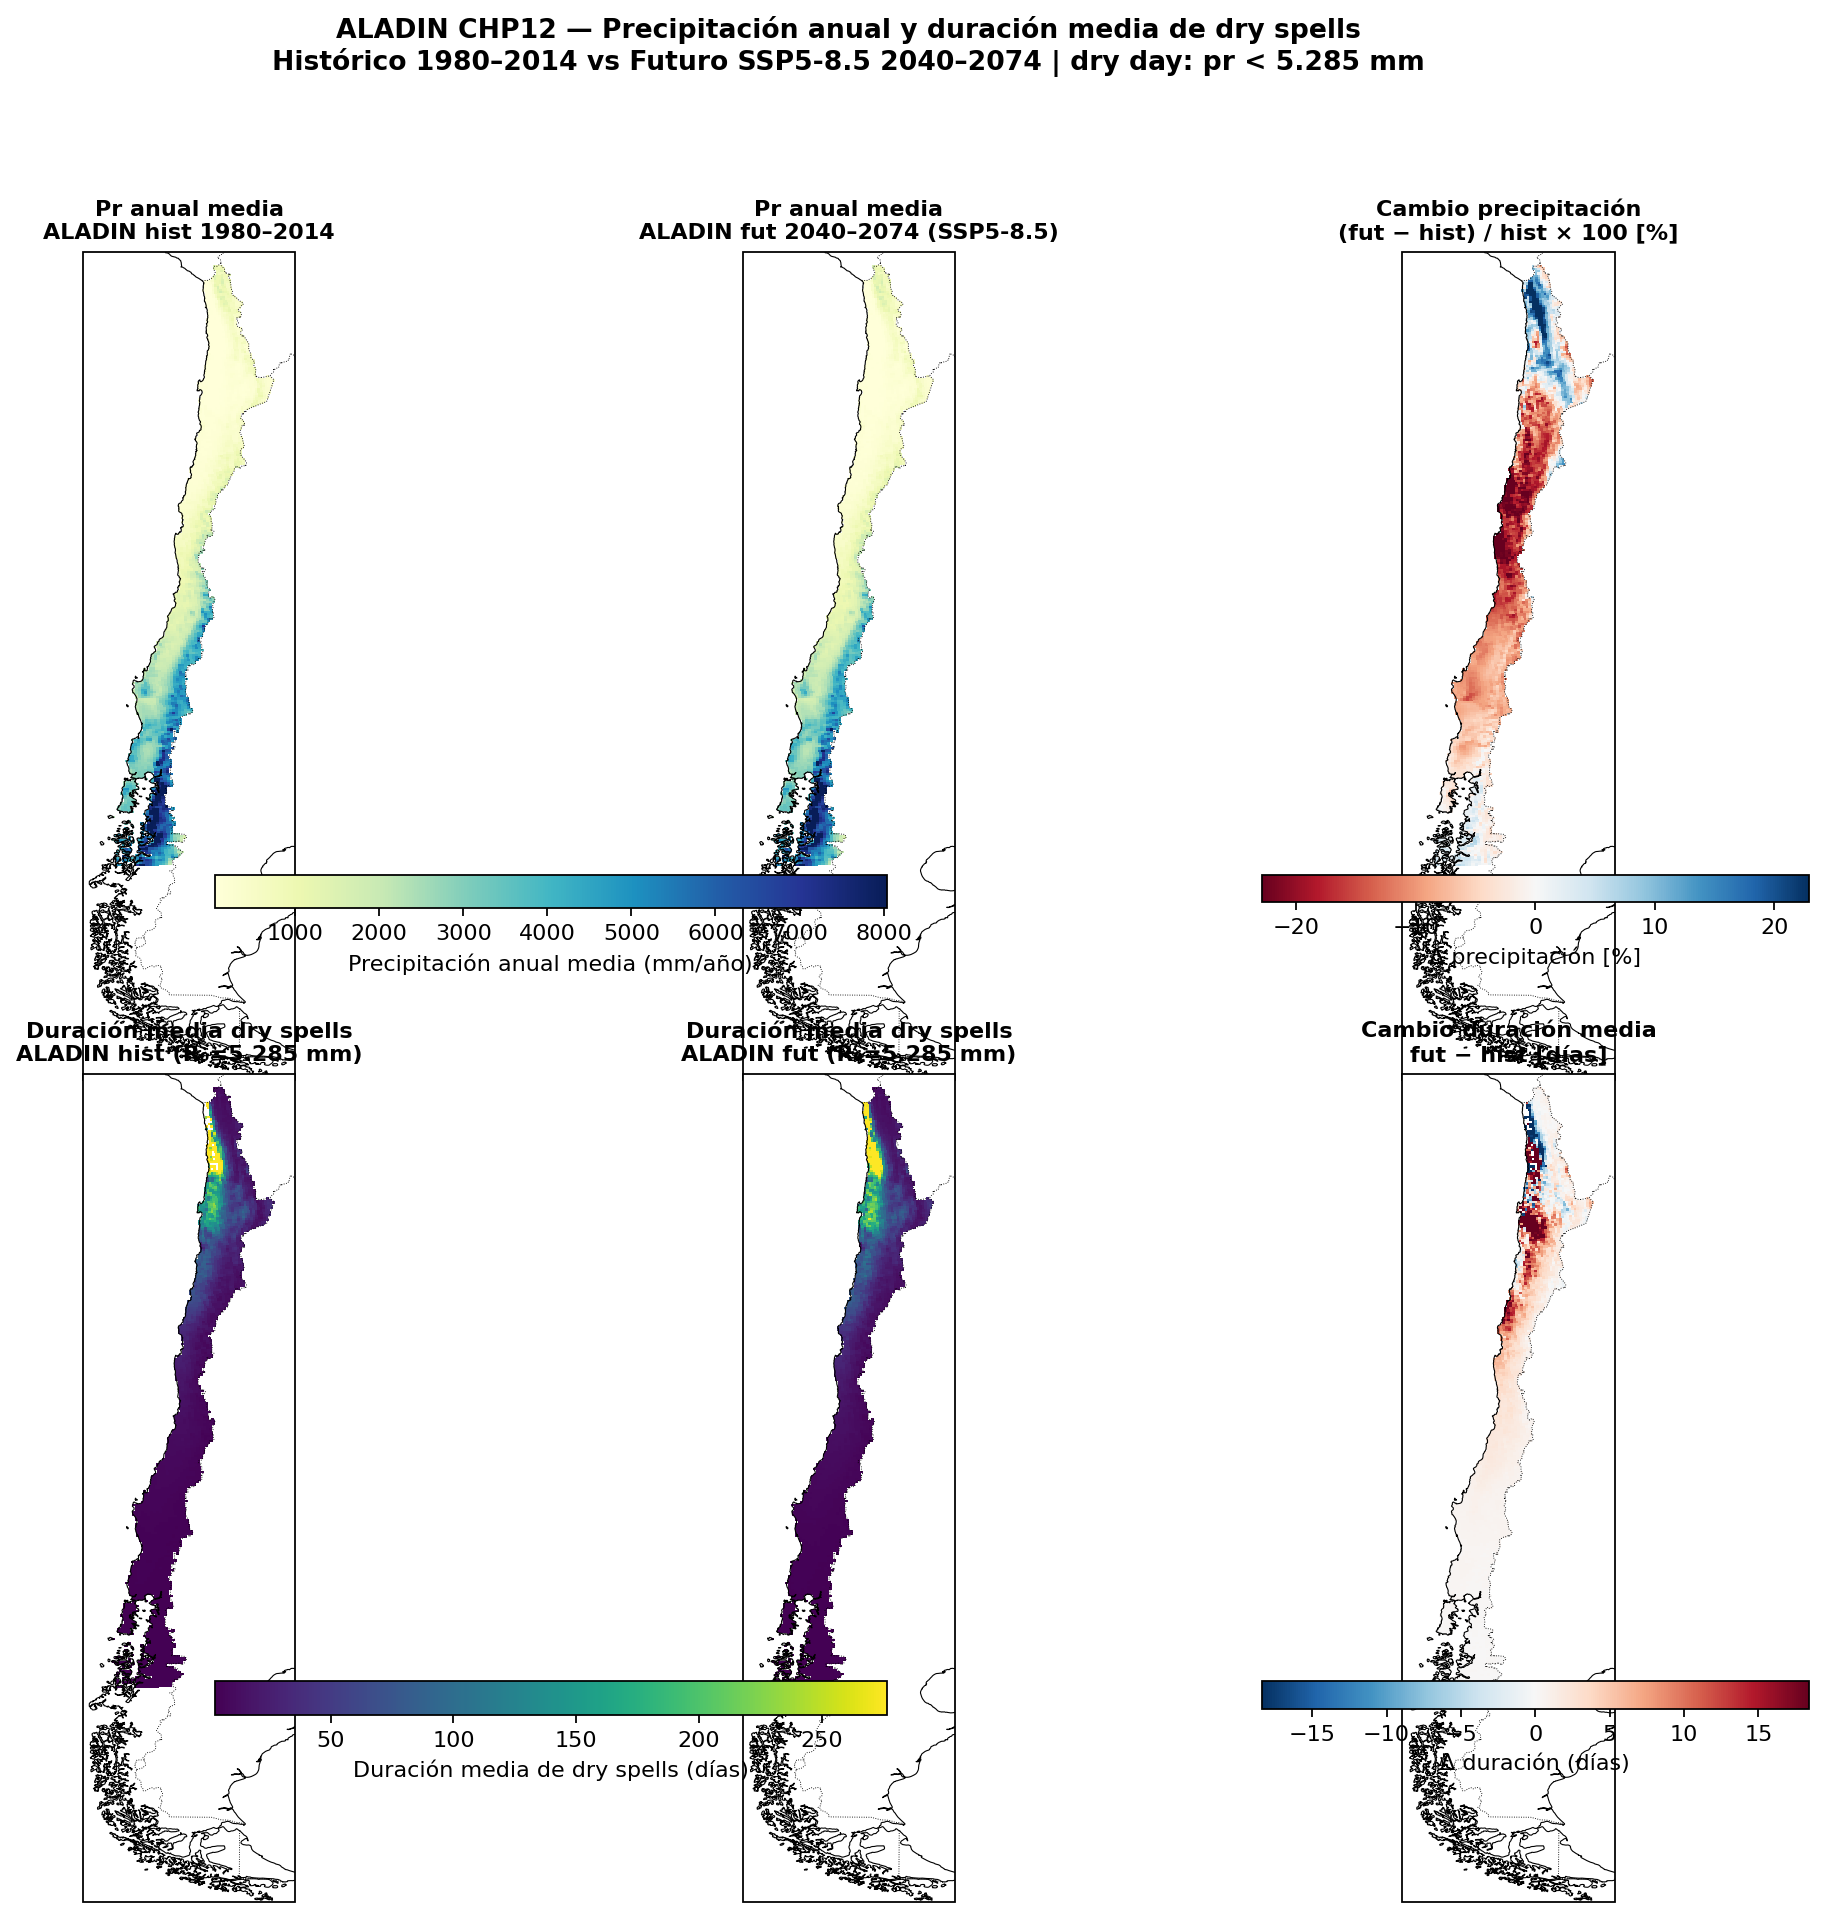
\includegraphics[width=1\linewidth,height=0.72\textheight,keepaspectratio,alt={ALADIN CHP12, criterio i. Fila superior: precipitación anual media en 1980--2014, 2040--2074 (SSP5-8.5) y cambio relativo (\%). Fila inferior: duración media de dry spells en ambos períodos y diferencia absoluta (días). El centro-sur pierde lluvia anual y alarga las rachas secas; no es un simple reescalado de la media de precipitación.}]{mapas_aladin_pr_anual_y_dryspells_hist_fut.png}
\caption[Precipitación anual y duración media de dry spells en ALADIN, histórico y futuro]{ALADIN CHP12, criterio i. Fila superior: precipitación anual media en 1980--2014, 2040--2074 (SSP5-8.5) y cambio relativo (\%). Fila inferior: duración media de dry spells en ambos períodos y diferencia absoluta (días). El centro-sur pierde lluvia anual y alarga las rachas secas; no es un simple reescalado de la media de precipitación.}\label{fig:mapas_futuro}
\end{figure}

\section{Risk ratios: más dry spells largos}\label{sec:rr_res}

El risk ratio RR(D) = N\_fut(t ≥ D) / N\_hist(t ≥ D) se estima en pools de regiones administrativas, con spells de inicio en marzo--noviembre y bootstrap por años (Figura~\ref{fig:rr}; Tabla~\ref{tab:rr}). A D = 20 días, Coquimbo pasa de 25 367 a 28 458 spells largos (RR = 1,12; IC95 {[}1,01, 1,25{]}); La Araucanía, de 2 397 a 4 118 (RR = 1,72; {[}1,10, 2,88{]}). En esas dos regiones el IC95 queda por completo sobre 1: el aumento es significativo. O'Higgins tiene RR = 1,15 (7 015 → 8 096), pero el IC95 {[}0,95, 1,40{]} cruza 1; aunque el RR es mayor que 1 en toda la cola, el intervalo solo queda marginalmente sobre 1 a D = 60 días (RR = 1,49; {[}1,01, 2,22{]}), por lo que no se interpreta como un aumento robusto. Los Lagos tiene RR = 2,15 (601 → 1 291), pero el IC95 {[}0,90, 8,50{]} cruza 1: el cociente es inestable porque los spells ≥ 20 días son raros en el histórico.

La señal no es un desplazamiento uniforme de toda la distribución. En Coquimbo, a D = 5 días el RR de conteos es 0,94 (IC95 por debajo de 1): hay menos spells cortos, coherente con la caída de n\_spells. El aumento es significativo a D = 20 días y de forma sostenida entre 30 y 60 días (p.~ej. RR = 1,26 a D = 30 días, IC95 {[}1,10, 1,43{]}). En La Araucanía el RR crece con D y alcanza 3,47 a 30 días, con IC95 amplio ({[}1,29, 11,8{]}): hay más ocurrencia de spells largos, pero la rareza histórica infla el cociente. Eso es lo que un CDD anual no muestra: el cambio está en la frecuencia de excedencias a lo largo de la cola, no en un único máximo por año (Sillmann et al., 2013b; Wainwright et al., 2021).

\begin{longtable}[]{@{}cccccc@{}}
\caption[Risk ratio a D = 20 días por región (SSP5-8.5)]{Risk ratio a D = 20 días. RR = N\_fut(t ≥ 20) / N\_hist(t ≥ 20). ALADIN, R₀ = 5,285 mm, inicio marzo--noviembre. IC95 por bootstrap de años (1 000 réplicas).}\label{tab:rr}\tabularnewline
\toprule\noalign{}
Región & N\_hist (t≥20) & N\_fut (t≥20) & RR & IC95 & ¿Aumento sig.? \\
\midrule\noalign{}
\endfirsthead
\toprule\noalign{}
Región & N\_hist (t≥20) & N\_fut (t≥20) & RR & IC95 & ¿Aumento sig.? \\
\midrule\noalign{}
\endhead
\bottomrule\noalign{}
\endlastfoot
Coquimbo & 25367 & 28458 & 1,12 & {[}1,01, 1,25{]} & Sí \\
O'Higgins & 7015 & 8096 & 1,15 & {[}0,95, 1,40{]} & No (IC cruza 1) \\
La Araucanía & 2397 & 4118 & 1,72 & {[}1,10, 2,88{]} & Sí \\
Los Lagos & 601 & 1291 & 2,15 & {[}0,90, 8,50{]} & No (IC cruza 1) \\
\end{longtable}

\begin{figure}[htbp]
\centering
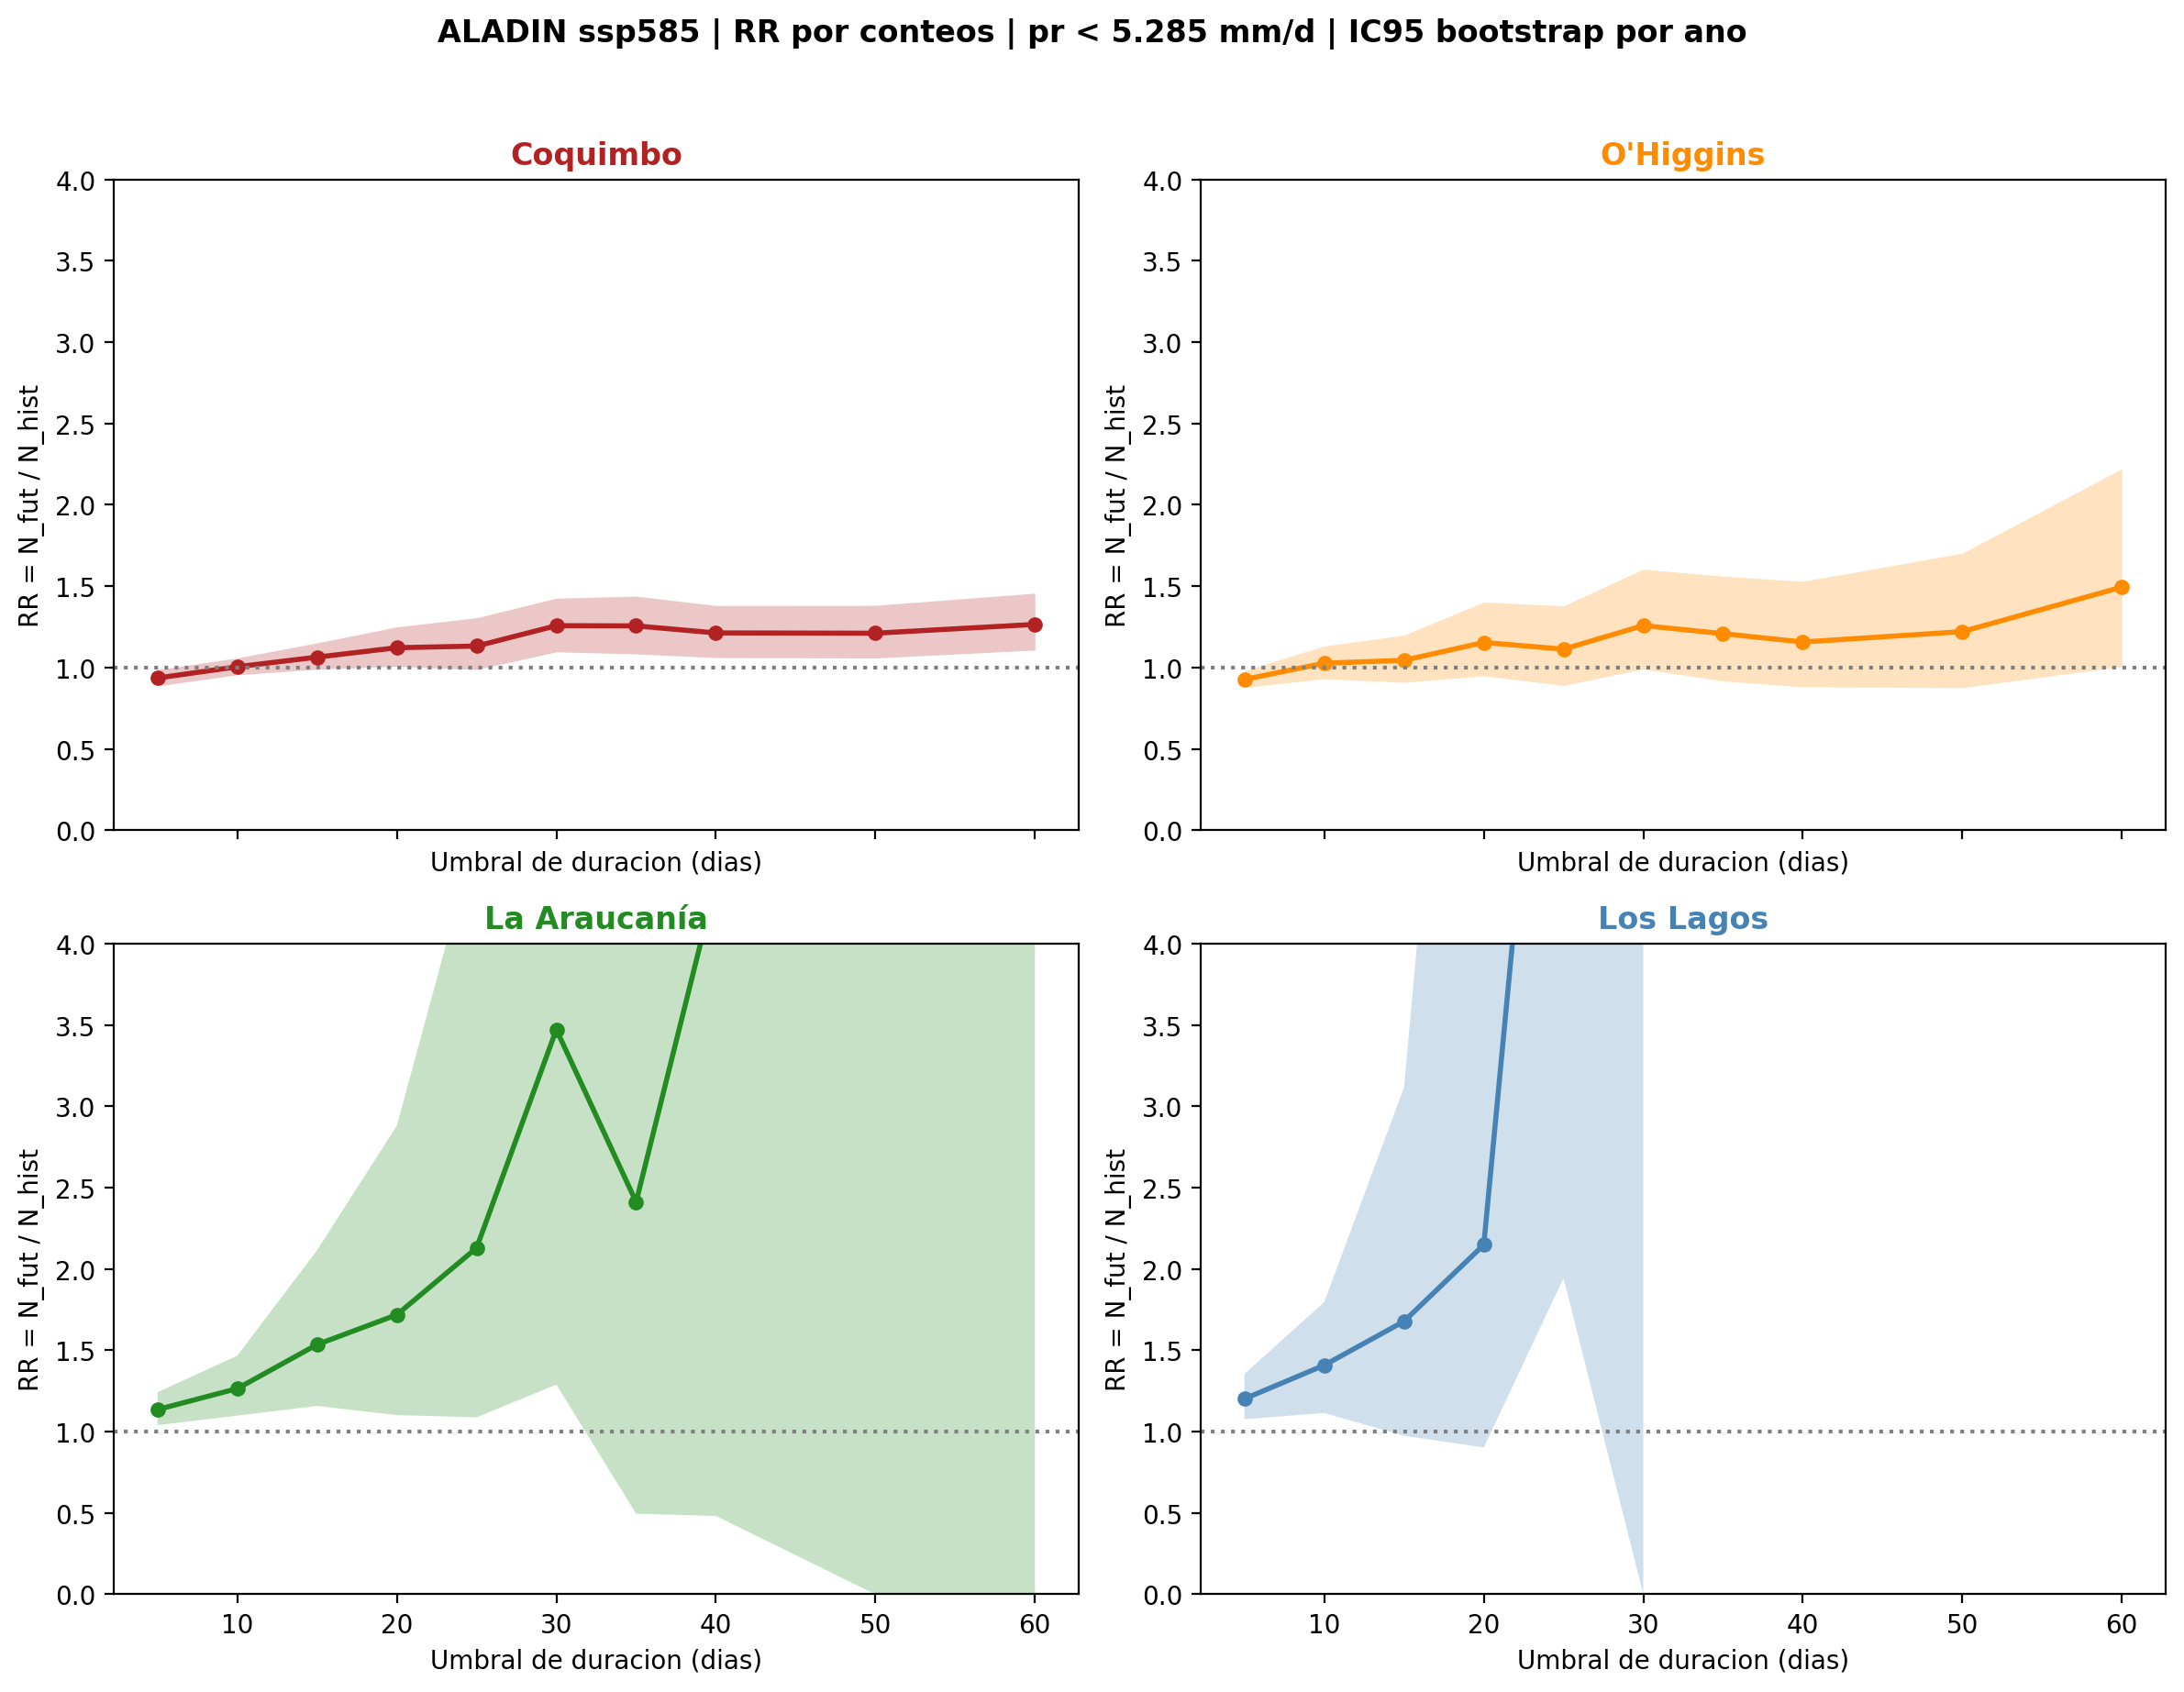
\includegraphics[width=1\linewidth,height=0.72\textheight,keepaspectratio,alt={Risk ratio RR(D) = N\_fut(t ≥ D) / N\_hist(t ≥ D) de dry spells con duración al menos D días. ALADIN, SSP5-8.5 (2040--2074) respecto de 1980--2014, R₀ = 5,285 mm, inicio marzo--noviembre. La banda es el IC95 por bootstrap de años. La línea punteada marca RR = 1. Coquimbo y La Araucanía superan 1 con IC que no cruza 1 a D = 20 días; O'Higgins y Los Lagos no. En el sur la banda se abre cuando D crece y los eventos históricos escasean.}]{fig08_rr_curves_aladin.png}
\caption[Risk ratio RR(D) = N\_fut(t ≥ D) / N\_hist(t ≥ D) de dry spells con duración al menos D días]{Risk ratio RR(D) = N\_fut(t ≥ D) / N\_hist(t ≥ D) de dry spells con duración al menos D días. ALADIN, SSP5-8.5 (2040--2074) respecto de 1980--2014, R₀ = 5,285 mm, inicio marzo--noviembre. La banda es el IC95 por bootstrap de años. La línea punteada marca RR = 1. Coquimbo y La Araucanía superan 1 con IC que no cruza 1 a D = 20 días; O'Higgins y Los Lagos no. En el sur la banda se abre cuando D crece y los eventos históricos escasean.}\label{fig:rr}
\end{figure}

\section{PDFs por cuenca: extensión de la cola futura}\label{sec:pdfs_fut}

Las PDFs de la Figura~\ref{fig:pdfs}, leídas ahora en la curva futura, muestran el cambio de forma y de n\_spells. En las cuatro cuencas el futuro de ALADIN tiene menos spells que el histórico: hay menos interrupciones y, por tanto, rachas más largas. La señal es clara en Maipo--Maule--Biobío, donde suben la media y el p99 y la cola se extiende hacia duraciones de decenas a cientos de días; en Loa el cambio relativo es menor porque las rachas ya son prolongadas (Tabla~\ref{tab:estadisticos}; Figura~\ref{fig:pdfs}). En escala log--log las curvas no son una traslación paralela: el exceso futuro se concentra a la derecha.

El máximo muestral es un estadístico ruidoso y no debe usarse solo. En Biobío, por ejemplo, el máximo del pool baja aunque media, p90, p99 y la probabilidad de spells ≥ 20 días suben. Eso ilustra por qué el objeto del trabajo es la distribución y las excedencias, no el récord de un píxel.

En conjunto, los risk ratios y las distribuciones de duración muestran un alargamiento de los dry spells hacia mediados de siglo, concentrado especialmente en la cola en Chile central y centro-sur. El cambio relativo es pequeño en Loa, donde las rachas ya son prolongadas en el histórico, mientras que en Los Lagos la estimación de la cola permanece incierta por la rareza de eventos largos.

\pendiente{decidir si las sensibilidades S4 (umbral) y S6 (SSP3-7.0) del Anexo A se
integran aquí como sección de robustez.}

\chapter{Discusión}\label{cap:6}

\section{Síntesis e interpretación}\label{sec:sintesis}

Tras igualar la frecuencia de días húmedos (criterio i), ALADIN reproduce el gradiente norte--sur de persistencia de CR2MET, pero subestima la duración de los dry spells, sobre todo en la cola (t99). La calibración de R₀ corrige gran parte del sesgo asociado al exceso de días con precipitación débil, un problema persistente en modelos climáticos, que tienden a llover con demasiada frecuencia y poca intensidad (Sun et al., 2006; Stephens et al., 2010; Chen et al., 2021; Martinez-Villalobos et al., 2022). Sin embargo, no elimina las diferencias en duración. Igualar la frecuencia de días húmedos es, por tanto, necesario pero no suficiente: también importa cómo se organizan esos días en el tiempo y cuánto fragmentan las rachas secas. Este sesgo de cola es coherente con Petrova et al.~(2024), quienes encuentran que la mayoría de los modelos CMIP5 y CMIP6 subestiman la racha seca anual más larga observada y que los modelos que la subestiman en el histórico tienden a proyectar aumentos futuros menores. Aunque esa relación se obtuvo con modelos globales y un indicador anual, sugiere que el alargamiento proyectado por ALADIN podría ser conservador, especialmente en el norte árido, donde el acortamiento de la cola histórica es mayor.

Hacia 2040--2074 bajo SSP5-8.5, ALADIN proyecta menos dry spells, pero más largos: aumenta el número de rachas de 20 días o más, con señal significativa en Coquimbo y La Araucanía, y las PDFs de Maipo, Maule y Biobío extienden la cola. Esta reorganización es opuesta a la que Latoja et al.~(2025) documentan con CR2MET en Chile central (32°--40°S) entre 1960 y 2021: más dry spells, pero más cortos, junto con menos precipitación por racha húmeda. Ambos resultados describen un secado, pero no la misma reorganización temporal. En el registro observado, la disminución de precipitación se expresa sobre todo en eventos húmedos más débiles e intermitentes. En la proyección, se expresa en menos interrupciones de los períodos secos, coherente con el papel dominante del aumento de días secos en el secado proyectado para climas mediterráneos (Polade et al., 2014, 2017). Parte del contraste puede deberse al forzante: la megasequía combina variabilidad interna con una contribución antrópica (Boisier et al., 2016; Garreaud et al., 2020), mientras que bajo SSP5-8.5 domina la respuesta forzada. También difieren la métrica y la ventana: Latoja et al.~analizan la tendencia de la duración media en seis décadas, y aquí se compara la cola entre dos períodos de 35 años. Secarse, por tanto, no implica una única forma de reorganizar las rachas secas, y el cambio en su duración no puede inferirse solo del signo del cambio en la precipitación total.

\section{Implicaciones para evaluación de modelos y riesgo de sequía}\label{sec:implicaciones}

Los resultados históricos tienen una implicación directa para la evaluación de RCMs en climas mediterráneos y áridos. Validar la precipitación media o la frecuencia de días húmedos no basta para juzgar la persistencia seca: aun después de igualar esa frecuencia, ALADIN acorta las rachas y, sobre todo, su cola. Una evaluación orientada a sequía debería, por tanto, comparar la distribución de duraciones tras controlar la frecuencia de días húmedos (Leung et al., 2022) y reportar explícitamente la cola. Esto importa también para las proyecciones: si, como encuentran Petrova et al.~(2024), los modelos que subestiman las rachas largas históricas tienden a proyectar aumentos menores, el sesgo de cola histórico condiciona cuánto confiar en la magnitud del cambio futuro. La metodología, basada en PDFs que conservan el número de spells, risk ratios de conteos y calibración previa de días húmedos, es transferible a otros RCMs del dominio CHP.

Para la gestión hídrica y la agricultura, el resultado central es que el cambio proyectado se concentra en las rachas largas y no se deduce del cambio en la precipitación total. Un aumento en el número de rachas de 20 días o más puede tener consecuencias que la reducción de la precipitación anual no anticipa, porque los períodos prolongados sin lluvia condicionan el déficit de humedad del suelo, la recarga y la planificación del riego. Un índice como el CDD, que retiene un solo extremo por año, tampoco captura ese cambio, que se distribuye a lo largo de la cola.

\section{Limitaciones y perspectivas}\label{sec:limitaciones}

Varias limitaciones acotan la interpretación. Primera, se usa un único RCM y un único escenario de altas emisiones; los cambios proyectados describen la respuesta de ALADIN bajo SSP5-8.5, no la incertidumbre multimodelo. Segunda, el umbral R₀ calibrado en el histórico se aplica también al futuro, lo que supone que el sesgo de frecuencia de días húmedos del modelo no cambia con el clima. Tercera, los píxeles de un mismo pool no son independientes, de modo que el número de spells sobrestima la información independiente; por eso la incertidumbre se estima remuestreando años y no spells individuales. Cuarta, en el norte árido ALADIN acorta la cola respecto de CR2MET incluso tras calibrar R₀, de modo que la frecuencia absoluta de spells muy largos en Loa debe leerse como conservadora. Quinta, en regiones muy húmedas como Los Lagos, los RR para umbrales altos son inestables: los pocos eventos históricos producen intervalos de confianza amplios aunque el cociente puntual sea alto. Finalmente, el trabajo caracteriza la reorganización de las rachas secas, pero no diagnostica los mecanismos de circulación que la producen.

El trabajo futuro puede avanzar en tres direcciones. La primera es extender el análisis a otros RCMs del dominio CHP y a otros escenarios, lo que permitiría además evaluar si, como sugieren Petrova et al.~(2024), los modelos con mayor sesgo de cola histórico proyectan aumentos menores. La segunda es evaluar si ALADIN reproduce la tendencia observada hacia spells más numerosos y más cortos en Chile central (Latoja et al., 2025), y vincular el contraste con el futuro a cambios en la circulación. La tercera es relacionar las PDFs de duración con índices de sequía y caudales, para traducir el cambio en la cola a impactos hidrológicos.

Los resultados muestran que el secado futuro proyectado por ALADIN no consiste únicamente en una reducción de la precipitación acumulada. El modelo proyecta una reorganización temporal hacia menos interrupciones y rachas secas más prolongadas, con cambios particularmente visibles en la cola de la distribución en Chile central y centro-sur. Caracterizar esa persistencia permite identificar una dimensión del cambio hidroclimático que queda parcialmente oculta en la precipitación media y en índices basados en un único extremo anual.

\pendiente{ampliar con más literatura, posibles mecanismos de circulación, el papel
de los aerosoles en SSP3-7.0 y las implicancias para la gestión.}

\chapter{Conclusiones}\label{cap:7}

\pendiente{capítulo nuevo. Responder cada objetivo específico en un párrafo.
Viñetas de partida:}

\begin{itemize}
\tightlist
\item
  \textbf{Objetivo 1:} CR2MET muestra un gradiente norte--sur marcado: rachas medias de 65,6 días en Loa frente a 6,2 días en Biobío, con colas de cientos de días en el norte.
\item
  \textbf{Objetivo 2:} igualar la frecuencia de días húmedos es necesario, pero no suficiente: ALADIN reproduce el patrón espacial, pero acorta las rachas, sobre todo en la cola (Δ media −8,2 días; Δ t99 −46,3 días).
\item
  \textbf{Objetivo 3:} hacia 2040--2074, ALADIN proyecta menos rachas, pero más largas; el número de rachas de al menos 20 días aumenta en las cuatro regiones (significativo en Coquimbo y La Araucanía).
\item
  \textbf{Objetivo 4:} la evaluación histórica es robusta al regrillado, y la dirección de la señal futura se mantiene con otro umbral y con SSP3-7.0.
\item
  \textbf{Mensaje general:} el secado proyectado es una reorganización temporal hacia períodos secos más persistentes, que no se deduce del cambio en la precipitación total.
\item
  \textbf{Trabajo futuro:} otros RCM del dominio CHP, horizontes de fin de siglo, mecanismos de circulación e impactos hidrológicos.
\end{itemize}


\pendiente{agregar Stechmann y Neelin (2014), Sun et al.~(2006) y Chen et
al.~(2021); ordenar alfabéticamente; agregar las referencias nuevas del
Capítulo 2 y las citas de CR2MET y de ALADIN CHP12.}

\nocite{*}
\bibliographystyle{apalike}
\bibliography{referencias}

\appendix
\chapter{Material suplementario}\label{anx:A}

Este anexo complementa la sección 3.7. Reúne las pruebas de sensibilidad a la elección del umbral de día húmedo: (i) el sesgo histórico de ALADIN respecto de CR2MET en Chile continental con los tres criterios de la Tabla~\ref{tab:criterios} (Tabla~\ref{tab:S1}); (ii) las PDFs históricas por cuenca con cuatro definiciones de umbral (Tabla~\ref{tab:S2}, Figura~\ref{fig:S1}); (iii) el mapa de R₀ local (Figura~\ref{fig:S2}), y (iv) los risk ratios futuros recalculados con 1 mm en ALADIN (Tabla~\ref{tab:S3}, Figura~\ref{fig:S3}). Salvo que se indique lo contrario, se aplican las mismas reglas que en el artículo: período histórico 1980--2014, futuro 2040--2074 (SSP5-8.5), CR2MET interpolado a la grilla de ALADIN, máscara de Chile continental y exclusión de las rachas que tocan el inicio o el fin del período.

\section{Sensibilidad del sesgo histórico a la elección del umbral}\label{sec:S1}

La Tabla~\ref{tab:S1} repite el análisis de mapas de §\ref{sec:pool} con los tres criterios de umbral. Los valores son promedios espaciales sobre las celdas con al menos 30 rachas en ambos productos; la significancia se evalúa con el bootstrap pareado por años de §\ref{sec:pool} (1000 réplicas, IC95).

\begin{longtable}[]{@{}
  >{\raggedright\arraybackslash}p{(\linewidth - 16\tabcolsep) * \real{0.1111}}
  >{\raggedright\arraybackslash}p{(\linewidth - 16\tabcolsep) * \real{0.1111}}
  >{\raggedright\arraybackslash}p{(\linewidth - 16\tabcolsep) * \real{0.1111}}
  >{\raggedright\arraybackslash}p{(\linewidth - 16\tabcolsep) * \real{0.1111}}
  >{\raggedright\arraybackslash}p{(\linewidth - 16\tabcolsep) * \real{0.1111}}
  >{\raggedright\arraybackslash}p{(\linewidth - 16\tabcolsep) * \real{0.1111}}
  >{\raggedright\arraybackslash}p{(\linewidth - 16\tabcolsep) * \real{0.1111}}
  >{\raggedright\arraybackslash}p{(\linewidth - 16\tabcolsep) * \real{0.1111}}
  >{\raggedright\arraybackslash}p{(\linewidth - 16\tabcolsep) * \real{0.1111}}@{}}
\caption[Duración media y t99 de las rachas secas en Chile continental (1980--2014) para CR2MET (1 mm) y ALADIN con cada criterio de umbral]{Duración media y t99 de las rachas secas en Chile continental (1980--2014) para CR2MET (1 mm) y ALADIN con cada criterio de umbral. Δ = ALADIN − CR2MET, calculado píxel a píxel y promediado sobre las celdas comunes. Las dos últimas columnas indican el porcentaje de celdas donde la diferencia es significativa.}\label{tab:S1}\tabularnewline
\toprule\noalign{}
\begin{minipage}[b]{\linewidth}\raggedright
Criterio
\end{minipage} & \begin{minipage}[b]{\linewidth}\raggedright
Métrica
\end{minipage} & \begin{minipage}[b]{\linewidth}\raggedright
CR2MET (días)
\end{minipage} & \begin{minipage}[b]{\linewidth}\raggedright
ALADIN (días)
\end{minipage} & \begin{minipage}[b]{\linewidth}\raggedright
Δ medio (días)
\end{minipage} & \begin{minipage}[b]{\linewidth}\raggedright
Δ mediano (días)
\end{minipage} & \begin{minipage}[b]{\linewidth}\raggedright
\% celdas ALADIN \textless{} CR2MET
\end{minipage} & \begin{minipage}[b]{\linewidth}\raggedright
\% celdas ALADIN \textgreater{} CR2MET
\end{minipage} & \begin{minipage}[b]{\linewidth}\raggedright
Celdas
\end{minipage} \\
\midrule\noalign{}
\endfirsthead
\toprule\noalign{}
\begin{minipage}[b]{\linewidth}\raggedright
Criterio
\end{minipage} & \begin{minipage}[b]{\linewidth}\raggedright
Métrica
\end{minipage} & \begin{minipage}[b]{\linewidth}\raggedright
CR2MET (días)
\end{minipage} & \begin{minipage}[b]{\linewidth}\raggedright
ALADIN (días)
\end{minipage} & \begin{minipage}[b]{\linewidth}\raggedright
Δ medio (días)
\end{minipage} & \begin{minipage}[b]{\linewidth}\raggedright
Δ mediano (días)
\end{minipage} & \begin{minipage}[b]{\linewidth}\raggedright
\% celdas ALADIN \textless{} CR2MET
\end{minipage} & \begin{minipage}[b]{\linewidth}\raggedright
\% celdas ALADIN \textgreater{} CR2MET
\end{minipage} & \begin{minipage}[b]{\linewidth}\raggedright
Celdas
\end{minipage} \\
\midrule\noalign{}
\endhead
\bottomrule\noalign{}
\endlastfoot
i: R₀ global (5,285 mm) & Duración media & 42,1 & 34,0 & −8,2 & −2,2 & 65,3 & 7,5 & 3526 \\
i: R₀ global (5,285 mm) & t99 & 221,1 & 175,3 & −46,3 & −17,2 & 42,6 & 3,5 & 3526 \\
ii: 1 mm en ambos & Duración media & 42,1 & 15,5 & −27,2 & −8,3 & 97,6 & 0,5 & 3549 \\
ii: 1 mm en ambos & t99 & 221,1 & 89,3 & −134,9 & −69,7 & 92,9 & 0,2 & 3549 \\
iii: R₀ local & Duración media & 42,1 & 35,3 & −6,8 & −1,9 & 48,9 & 0,2 & 3471 \\
iii: R₀ local & t99 & 221,1 & 184,0 & −36,0 & −6,5 & 26,0 & 4,4 & 3471 \\
\end{longtable}

Con el mismo umbral de 1 mm (criterio ii), ALADIN acorta las rachas en casi todo el país, porque produce demasiados días con lluvia débil que interrumpen las rachas. Al igualar la frecuencia de días húmedos con un umbral global (criterio i), el sesgo se reduce a menos de un tercio. El umbral local (criterio iii) lo reduce algo más, pero a escala nacional no lo elimina, especialmente en la cola (t99).

\section{PDFs históricas por cuenca con distintos umbrales}\label{sec:S2}

\begin{longtable}[]{@{}
  >{\raggedright\arraybackslash}p{(\linewidth - 14\tabcolsep) * \real{0.1250}}
  >{\raggedright\arraybackslash}p{(\linewidth - 14\tabcolsep) * \real{0.1250}}
  >{\raggedright\arraybackslash}p{(\linewidth - 14\tabcolsep) * \real{0.1250}}
  >{\raggedright\arraybackslash}p{(\linewidth - 14\tabcolsep) * \real{0.1250}}
  >{\raggedright\arraybackslash}p{(\linewidth - 14\tabcolsep) * \real{0.1250}}
  >{\raggedright\arraybackslash}p{(\linewidth - 14\tabcolsep) * \real{0.1250}}
  >{\raggedright\arraybackslash}p{(\linewidth - 14\tabcolsep) * \real{0.1250}}
  >{\raggedright\arraybackslash}p{(\linewidth - 14\tabcolsep) * \real{0.1250}}@{}}
\caption[Estadísticos de duración de las rachas secas por cuenca (1980--2014) para CR2MET con 1 mm y ALADIN con 1 mm (criterio ii), R₀ global (criterio i) y R₀ local (criterio iii)]{Estadísticos de duración de las rachas secas por cuenca (1980--2014) para CR2MET con 1 mm y ALADIN con 1 mm (criterio ii), R₀ global (criterio i) y R₀ local (criterio iii). n = número de rachas.}\label{tab:S2}\tabularnewline
\toprule\noalign{}
\begin{minipage}[b]{\linewidth}\raggedright
Cuenca
\end{minipage} & \begin{minipage}[b]{\linewidth}\raggedright
Serie
\end{minipage} & \begin{minipage}[b]{\linewidth}\raggedright
n
\end{minipage} & \begin{minipage}[b]{\linewidth}\raggedright
Media (días)
\end{minipage} & \begin{minipage}[b]{\linewidth}\raggedright
Mediana (días)
\end{minipage} & \begin{minipage}[b]{\linewidth}\raggedright
p90 (días)
\end{minipage} & \begin{minipage}[b]{\linewidth}\raggedright
p99 (días)
\end{minipage} & \begin{minipage}[b]{\linewidth}\raggedright
Máximo (días)
\end{minipage} \\
\midrule\noalign{}
\endfirsthead
\toprule\noalign{}
\begin{minipage}[b]{\linewidth}\raggedright
Cuenca
\end{minipage} & \begin{minipage}[b]{\linewidth}\raggedright
Serie
\end{minipage} & \begin{minipage}[b]{\linewidth}\raggedright
n
\end{minipage} & \begin{minipage}[b]{\linewidth}\raggedright
Media (días)
\end{minipage} & \begin{minipage}[b]{\linewidth}\raggedright
Mediana (días)
\end{minipage} & \begin{minipage}[b]{\linewidth}\raggedright
p90 (días)
\end{minipage} & \begin{minipage}[b]{\linewidth}\raggedright
p99 (días)
\end{minipage} & \begin{minipage}[b]{\linewidth}\raggedright
Máximo (días)
\end{minipage} \\
\midrule\noalign{}
\endhead
\bottomrule\noalign{}
\endlastfoot
Loa & CR2MET 1 mm & 55 015 & 65,6 & 23 & 185 & 456 & 1419 \\
Loa & ALADIN 1 mm & 129 292 & 27,0 & 12 & 70 & 206 & 1127 \\
Loa & ALADIN R₀ global & 66 267 & 54,6 & 22 & 143 & 360 & 1156 \\
Loa & ALADIN R₀ local & 71 662 & 50,5 & 21 & 127 & 353 & 1150 \\
Maipo & CR2MET 1 mm & 150 209 & 11,0 & 5 & 23 & 119 & 283 \\
Maipo & ALADIN 1 mm & 217 952 & 6,3 & 3 & 14 & 55 & 167 \\
Maipo & ALADIN R₀ global & 181 049 & 8,6 & 4 & 18 & 87 & 194 \\
Maipo & ALADIN R₀ local & 150 900 & 10,6 & 5 & 21 & 124 & 226 \\
Maule & CR2MET 1 mm & 184 462 & 9,5 & 5 & 21 & 83 & 206 \\
Maule & ALADIN 1 mm & 257 231 & 5,8 & 3 & 13 & 39 & 142 \\
Maule & ALADIN R₀ global & 228 077 & 7,3 & 4 & 17 & 57 & 160 \\
Maule & ALADIN R₀ local & 212 397 & 8,2 & 4 & 19 & 67 & 194 \\
Biobío & CR2MET 1 mm & 344 251 & 6,2 & 4 & 14 & 44 & 109 \\
Biobío & ALADIN 1 mm & 423 294 & 4,2 & 3 & 9 & 22 & 79 \\
Biobío & ALADIN R₀ global & 399 130 & 5,3 & 3 & 12 & 34 & 153 \\
Biobío & ALADIN R₀ local & 395 037 & 5,4 & 3 & 12 & 35 & 153 \\
\end{longtable}

\begin{figure}[htbp]
\centering
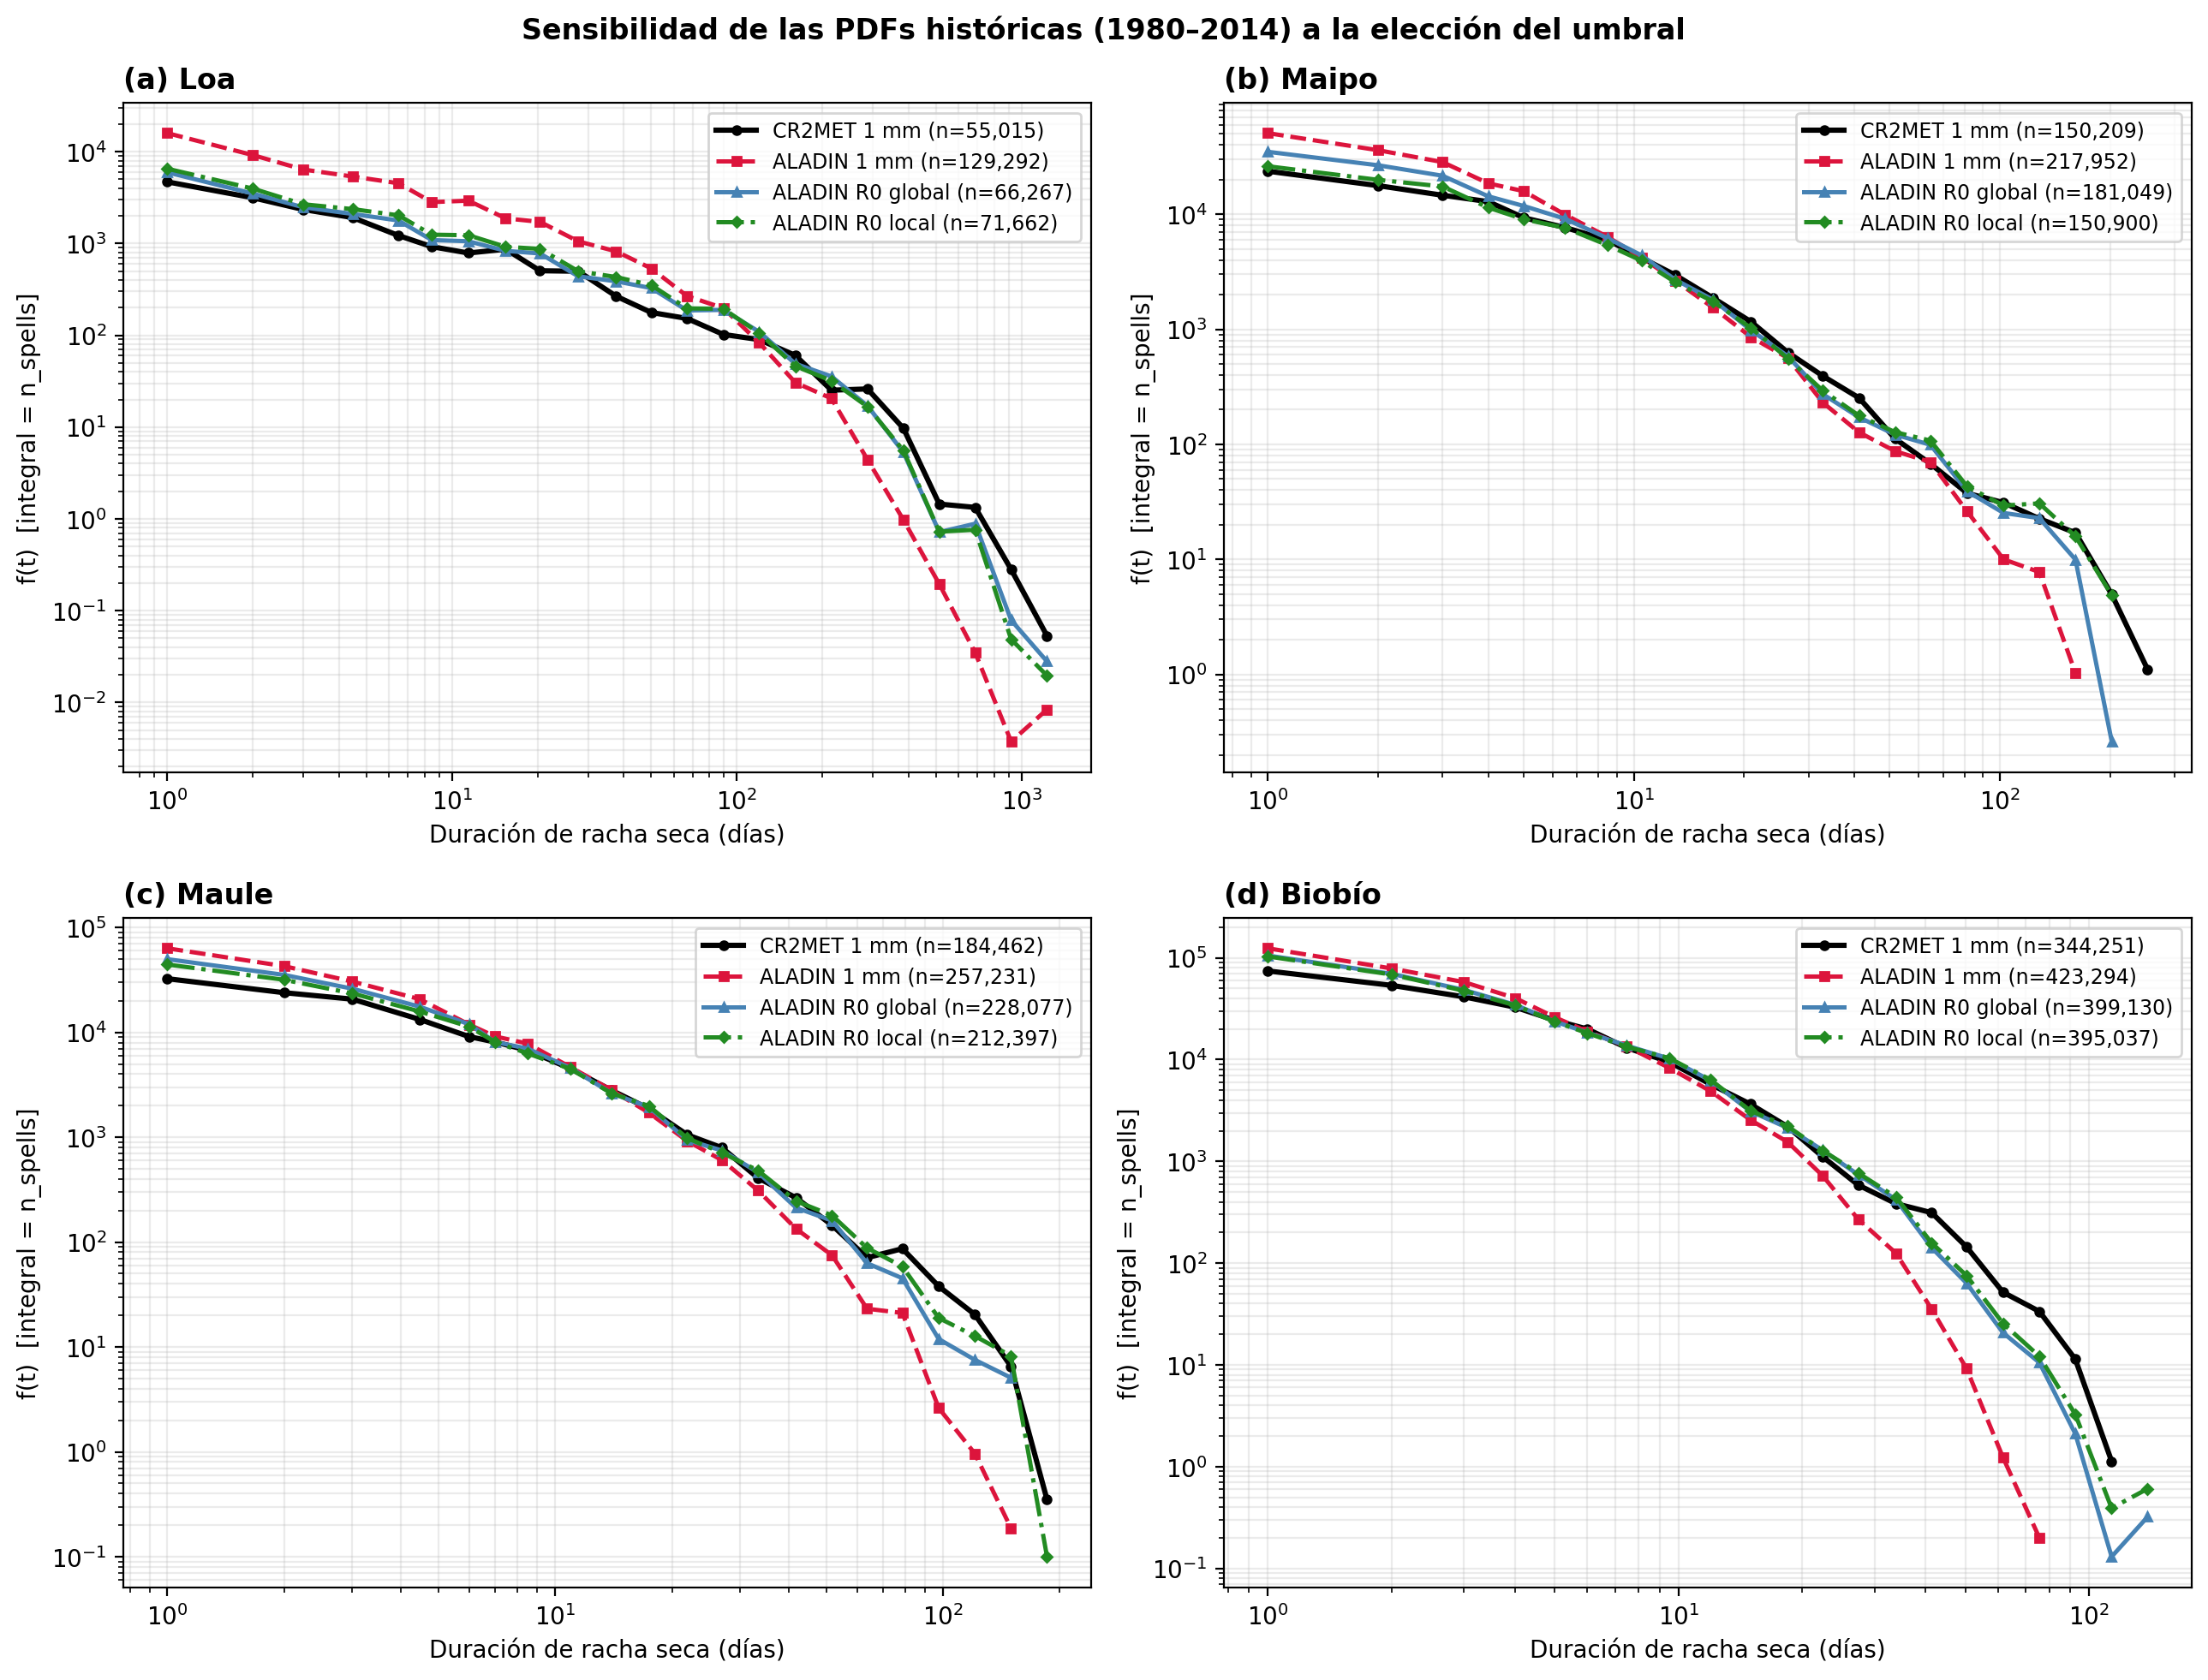
\includegraphics[width=1\linewidth,height=0.72\textheight,keepaspectratio,alt={Sensibilidad de las PDFs históricas (1980--2014) de duración de rachas secas a la elección del umbral de día húmedo, en las cuencas (a) Loa, (b) Maipo, (c) Maule y (d) Biobío. Se comparan CR2MET con 1 mm (negro) y ALADIN con 1 mm (criterio ii, rojo), con R₀ global = 5,285 mm (criterio i, azul) y con R₀ local por píxel (criterio iii, verde). Ejes logarítmicos; los bins son comunes a las cuatro series de cada cuenca (§\ref{sec:pdfs}) y la integral de cada curva es igual a su número de rachas (n).}]{figS1_sensibilidad_umbral_cuencas.png}
\caption[Sensibilidad de las PDFs históricas (1980--2014) de duración de rachas secas a la elección del umbral de día húmedo, en las cuencas (a) Loa, (b) Maipo, (c) Maule y (d) Biobío]{Sensibilidad de las PDFs históricas (1980--2014) de duración de rachas secas a la elección del umbral de día húmedo, en las cuencas (a) Loa, (b) Maipo, (c) Maule y (d) Biobío. Se comparan CR2MET con 1 mm (negro) y ALADIN con 1 mm (criterio ii, rojo), con R₀ global = 5,285 mm (criterio i, azul) y con R₀ local por píxel (criterio iii, verde). Ejes logarítmicos; los bins son comunes a las cuatro series de cada cuenca (§\ref{sec:pdfs}) y la integral de cada curva es igual a su número de rachas (n).}\label{fig:S1}
\end{figure}

Con 1 mm, ALADIN sobreestima las rachas cortas y subestima las largas en las cuatro cuencas. La calibración del umbral acerca las PDFs de ALADIN a la de CR2MET; en Loa, Maule y Biobío la cola de ALADIN sigue terminando antes que la de CR2MET, mientras que en Maipo el R₀ local prácticamente iguala la cola observada (p99 de 124 días frente a 119 días en CR2MET).

\section{Mapa de R₀ local}\label{sec:S3}

\begin{figure}[htbp]
\centering
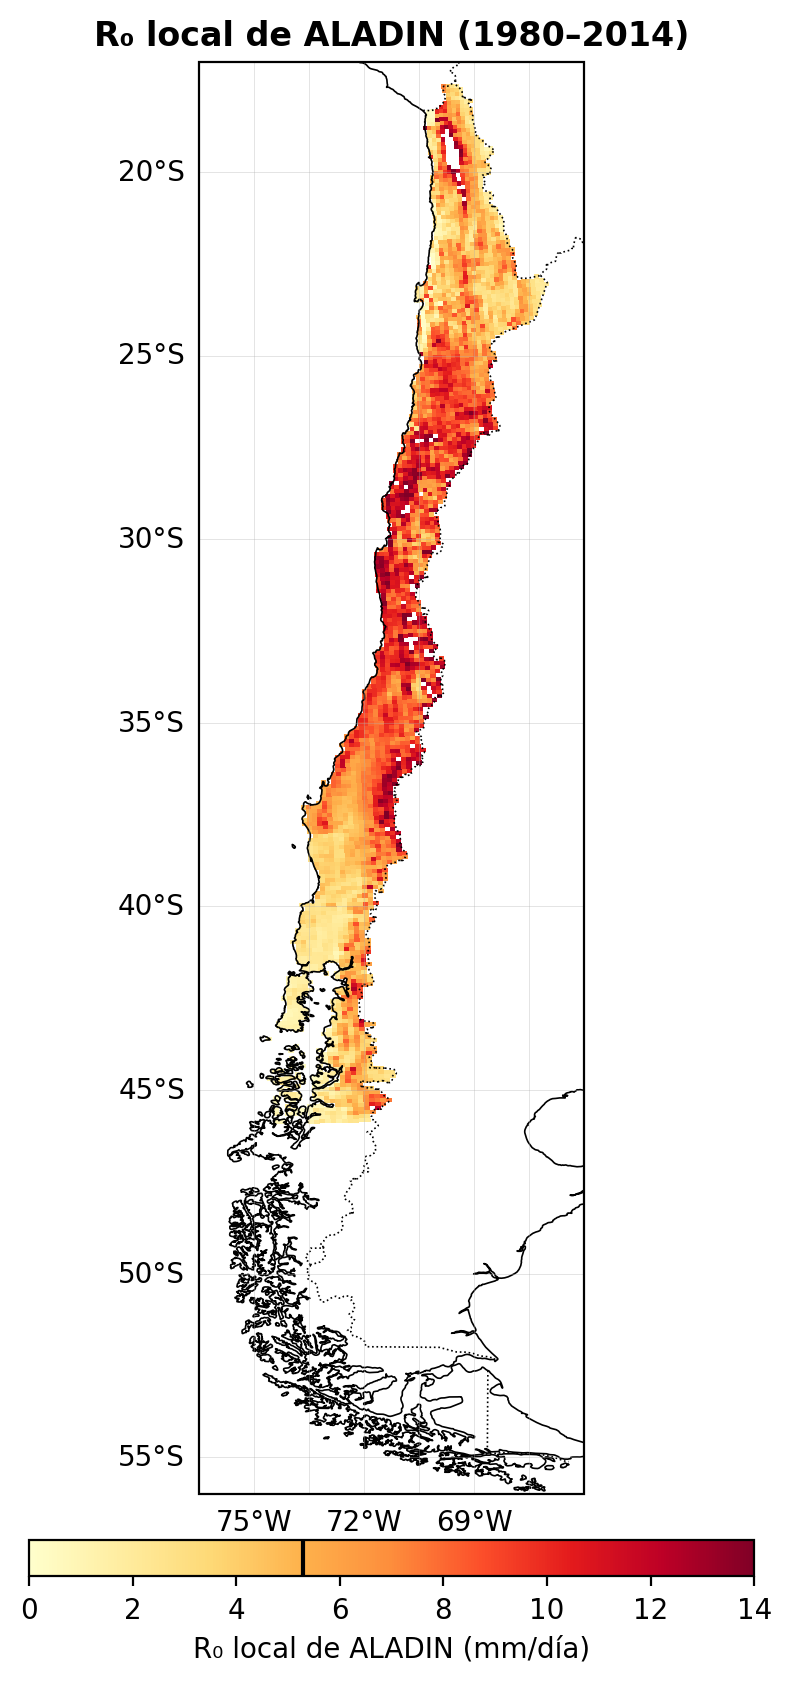
\includegraphics[width=1\linewidth,height=0.72\textheight,keepaspectratio,alt={Umbral local de día húmedo de ALADIN (R₀ local, criterio iii) en 1980--2014. En cada píxel, R₀ local es el umbral para el cual la fracción de días húmedos de ALADIN iguala la de CR2MET con 1 mm, obtenido por bisección. La línea negra en la barra de colores marca el R₀ global (5,285 mm). Los píxeles en blanco (82 de 3587) no tienen solución dentro del intervalo de búsqueda (0--15 mm).}]{figS2_mapa_R0_local.png}
\caption[Umbral local de día húmedo de ALADIN (R₀ local, criterio iii) en 1980--2014]{Umbral local de día húmedo de ALADIN (R₀ local, criterio iii) en 1980--2014. En cada píxel, R₀ local es el umbral para el cual la fracción de días húmedos de ALADIN iguala la de CR2MET con 1 mm, obtenido por bisección. La línea negra en la barra de colores marca el R₀ global (5,285 mm). Los píxeles en blanco (82 de 3587) no tienen solución dentro del intervalo de búsqueda (0--15 mm).}\label{fig:S2}
\end{figure}

El R₀ local tiene una mediana de 6,4 mm (p10 = 2,3 mm; p90 = 11,1 mm) y es inferior al R₀ global en el 39 \% de los píxeles. Los valores más altos se concentran en la zona centro-norte (aproximadamente 28--37 °S) y los más bajos en el extremo norte y en el sur. Esta heterogeneidad es la razón por la que el análisis principal usa un único umbral global (§\ref{sec:definicion}): corrige la frecuencia de días húmedos sin introducir un campo de umbrales que varía de un píxel a otro.

\section{Robustez de la señal futura al umbral}\label{sec:S4}

Para comprobar que el aumento futuro de rachas largas no es consecuencia de la calibración, los risk ratios de §\ref{sec:rr} se recalculan con 1 mm en ALADIN en ambos períodos, manteniendo todas las demás reglas (rachas iniciadas entre marzo y noviembre, bootstrap independiente por años, 1000 réplicas).

\begin{longtable}[]{@{}
  >{\raggedright\arraybackslash}p{(\linewidth - 8\tabcolsep) * \real{0.2000}}
  >{\raggedright\arraybackslash}p{(\linewidth - 8\tabcolsep) * \real{0.2000}}
  >{\raggedright\arraybackslash}p{(\linewidth - 8\tabcolsep) * \real{0.2000}}
  >{\raggedright\arraybackslash}p{(\linewidth - 8\tabcolsep) * \real{0.2000}}
  >{\raggedright\arraybackslash}p{(\linewidth - 8\tabcolsep) * \real{0.2000}}@{}}
\caption[Risk ratio RR(20) = N\_fut(t ≥ 20 d) / N\_hist(t ≥ 20 d) por región con R₀ global (análisis principal, Tabla~\ref{tab:rr}) y con 1 mm en ALADIN]{Risk ratio RR(20) = N\_fut(t ≥ 20 d) / N\_hist(t ≥ 20 d) por región con R₀ global (análisis principal, Tabla~\ref{tab:rr}) y con 1 mm en ALADIN. Entre corchetes, el IC95 bootstrap. En negrita, los aumentos significativos (IC95 completamente sobre 1).}\label{tab:S3}\tabularnewline
\toprule\noalign{}
\begin{minipage}[b]{\linewidth}\raggedright
Región
\end{minipage} & \begin{minipage}[b]{\linewidth}\raggedright
R₀ global: N\_hist → N\_fut
\end{minipage} & \begin{minipage}[b]{\linewidth}\raggedright
R₀ global: RR(20) {[}IC95{]}
\end{minipage} & \begin{minipage}[b]{\linewidth}\raggedright
1 mm: N\_hist → N\_fut
\end{minipage} & \begin{minipage}[b]{\linewidth}\raggedright
1 mm: RR(20) {[}IC95{]}
\end{minipage} \\
\midrule\noalign{}
\endfirsthead
\toprule\noalign{}
\begin{minipage}[b]{\linewidth}\raggedright
Región
\end{minipage} & \begin{minipage}[b]{\linewidth}\raggedright
R₀ global: N\_hist → N\_fut
\end{minipage} & \begin{minipage}[b]{\linewidth}\raggedright
R₀ global: RR(20) {[}IC95{]}
\end{minipage} & \begin{minipage}[b]{\linewidth}\raggedright
1 mm: N\_hist → N\_fut
\end{minipage} & \begin{minipage}[b]{\linewidth}\raggedright
1 mm: RR(20) {[}IC95{]}
\end{minipage} \\
\midrule\noalign{}
\endhead
\bottomrule\noalign{}
\endlastfoot
Coquimbo & 25 367 → 28 458 & \textbf{1,12 {[}1,01; 1,25{]}} & 18 366 → 22 266 & \textbf{1,21 {[}1,06; 1,39{]}} \\
O'Higgins & 7015 → 8096 & 1,15 {[}0,95; 1,40{]} & 4370 → 5132 & 1,17 {[}0,96; 1,47{]} \\
La Araucanía & 2397 → 4118 & \textbf{1,72 {[}1,10; 2,88{]}} & 360 → 1429 & \textbf{3,97 {[}1,46; 16,96{]}} \\
Los Lagos & 601 → 1291 & 2,15 {[}0,90; 8,50{]} & 107 → 27 & 0,25 {[}0,01; 28,07{]} \\
\end{longtable}

\begin{figure}[htbp]
\centering
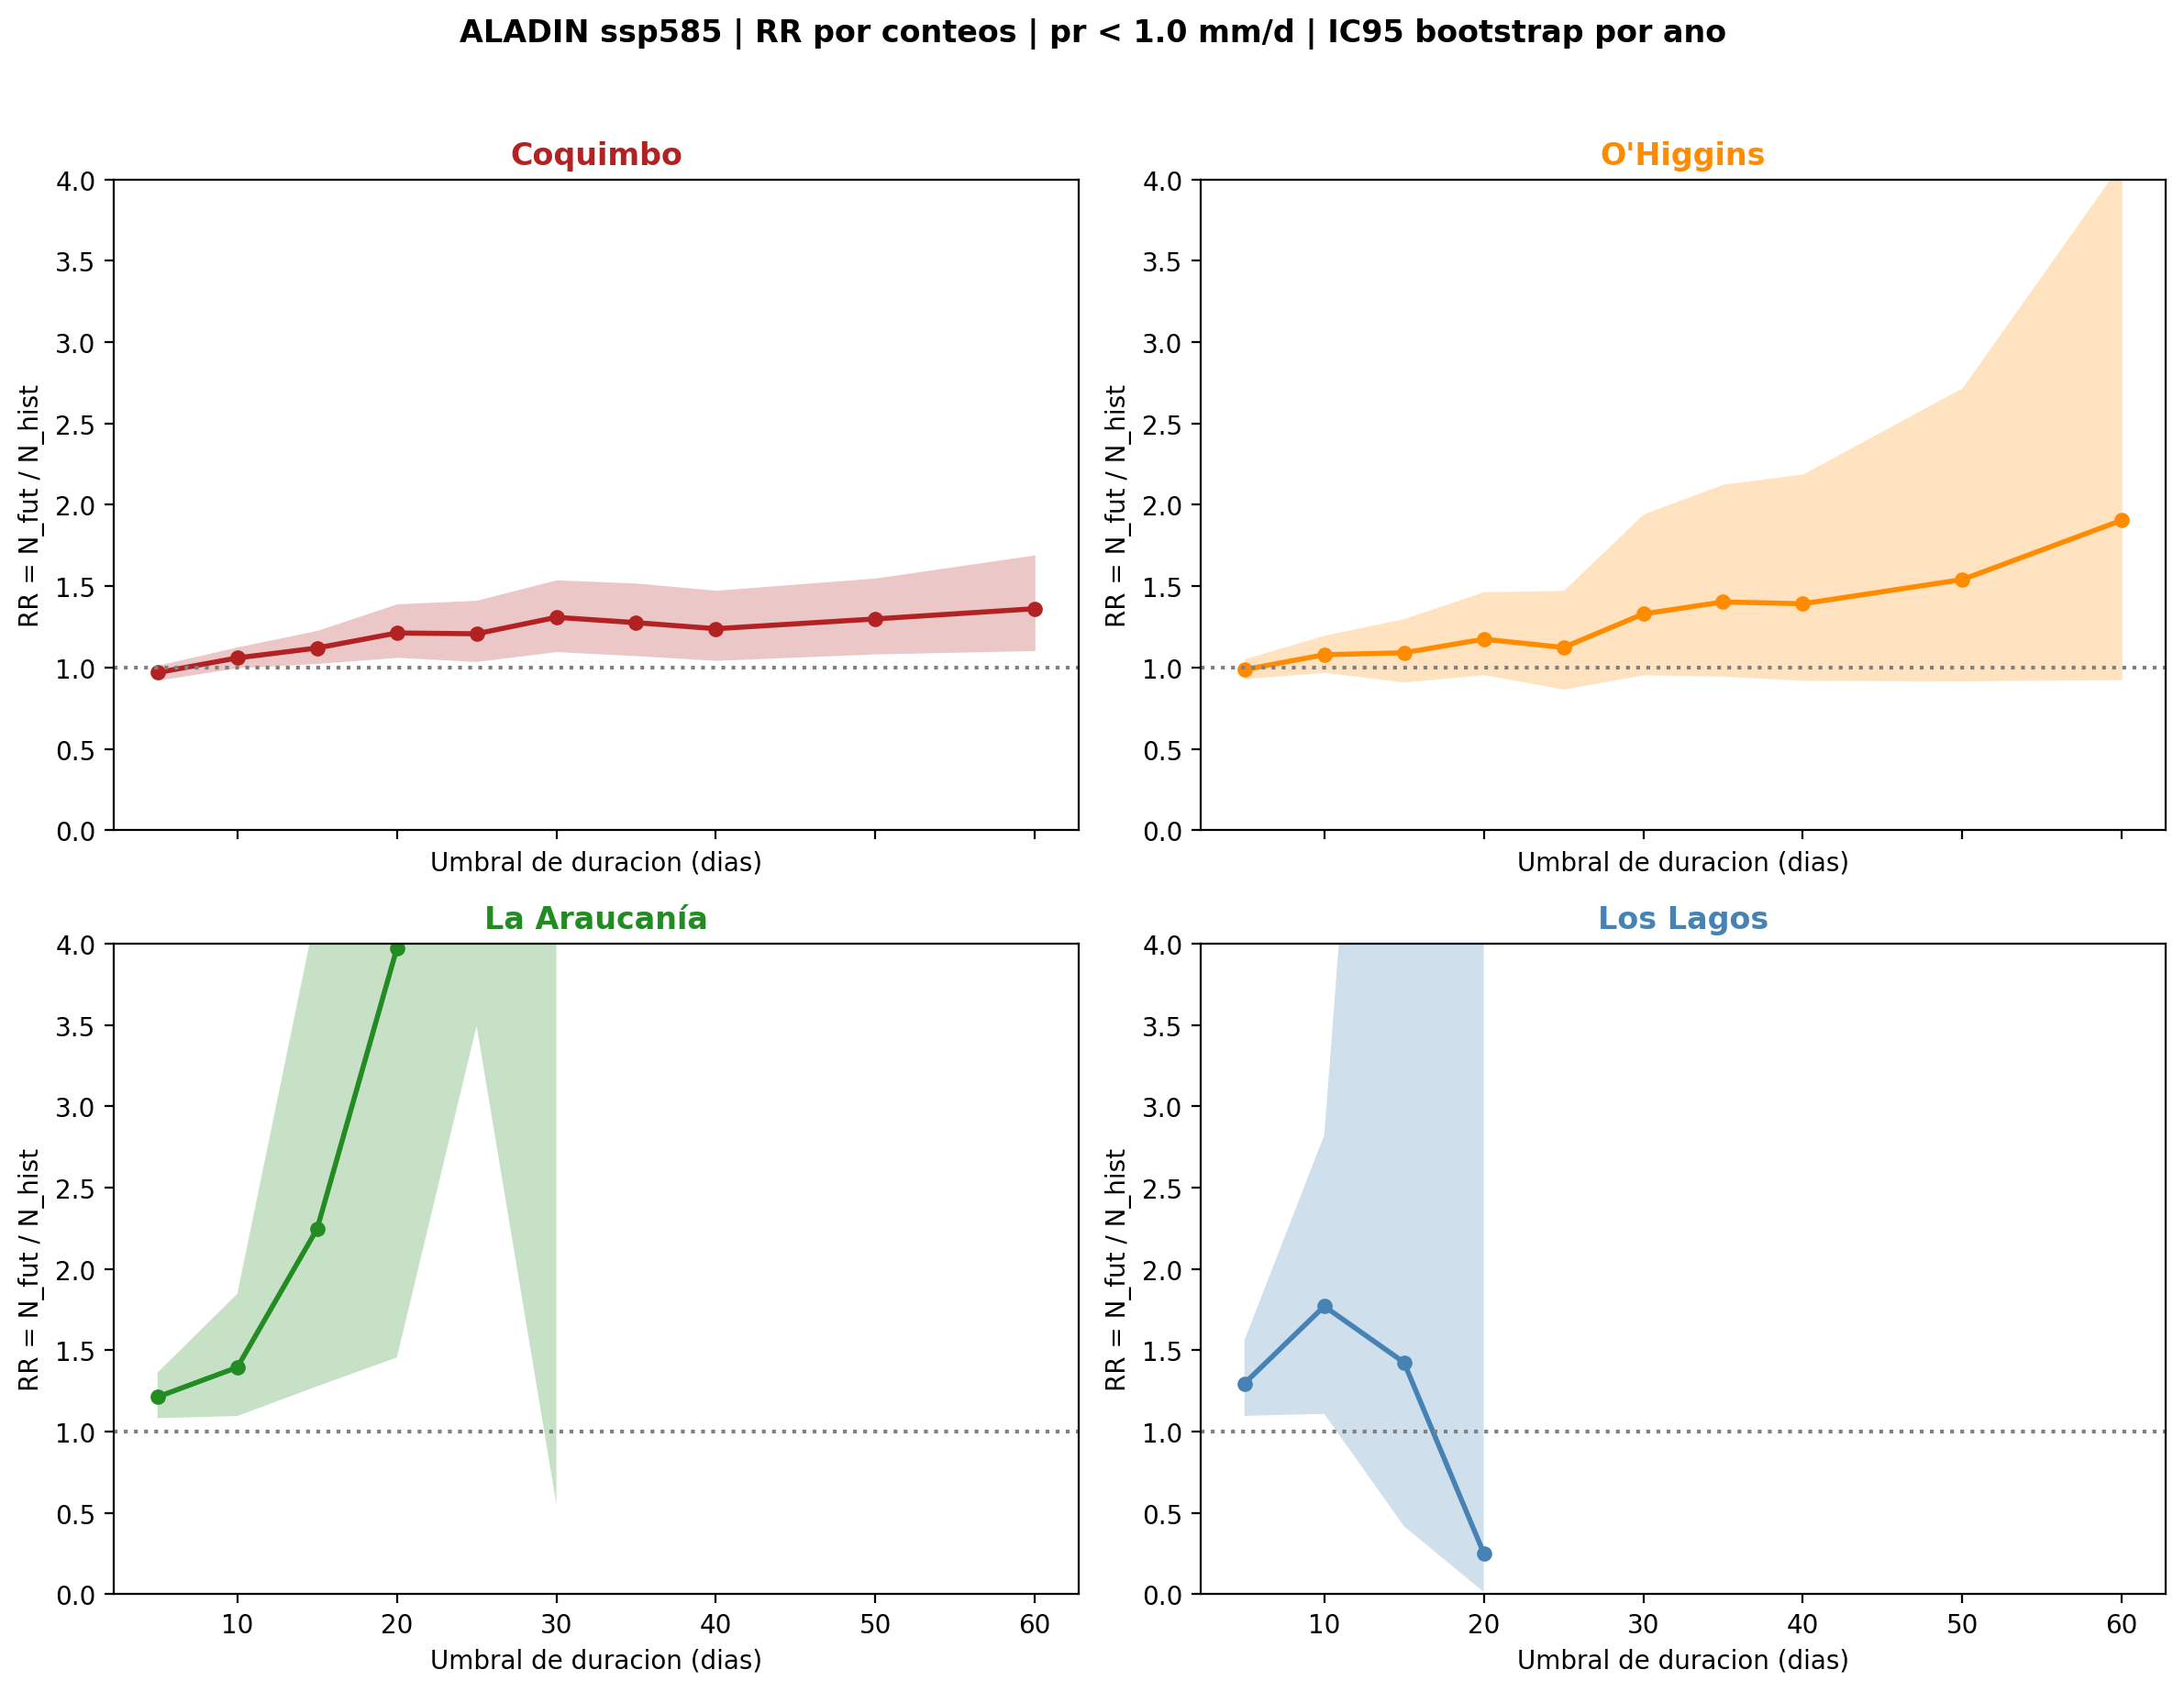
\includegraphics[width=1\linewidth,height=0.72\textheight,keepaspectratio,alt={Risk ratio RR(D) = N\_fut(t ≥ D) / N\_hist(t ≥ D) en función del umbral de duración D para las cuatro regiones, calculado con 1 mm en ALADIN (SSP5-8.5, 2040--2074 frente a 1980--2014). La banda sombreada es el IC95 bootstrap por años; la línea punteada marca RR = 1. Los puntos faltantes corresponden a umbrales sin rachas en el período histórico.}]{figS_rr_curves_aladin_1mm.png}
\caption[Risk ratio RR(D) = N\_fut(t ≥ D) / N\_hist(t ≥ D) en función del umbral de duración D para las cuatro regiones, calculado con 1 mm en ALADIN (SSP5-8.5, 2040--2074 frente a 1980--2014)]{Risk ratio RR(D) = N\_fut(t ≥ D) / N\_hist(t ≥ D) en función del umbral de duración D para las cuatro regiones, calculado con 1 mm en ALADIN (SSP5-8.5, 2040--2074 frente a 1980--2014). La banda sombreada es el IC95 bootstrap por años; la línea punteada marca RR = 1. Los puntos faltantes corresponden a umbrales sin rachas en el período histórico.}\label{fig:S3}
\end{figure}

Con 1 mm, el aumento de rachas largas se mantiene en Coquimbo, donde es significativo para todos los umbrales entre 15 y 60 días, y en La Araucanía. En O'Higgins el RR es mayor que 1 en casi todos los umbrales, pero el intervalo incluye 1, igual que en el análisis principal. En Los Lagos, ALADIN con 1 mm casi no produce rachas de 20 días o más (107 en 35 años), por lo que el RR(20) no es informativo; para duraciones cortas el aumento es significativo (RR(5) = 1,30 {[}1,10; 1,56{]}; RR(10) = 1,77 {[}1,11; 2,82{]}). La señal futura no depende, por lo tanto, de la calibración del umbral en las regiones donde hay rachas suficientes para evaluarla.

\section{Sensibilidad al método de regrillado de CR2MET}\label{sec:S5}

En el análisis principal, CR2MET se interpola linealmente a los centros de celda de ALADIN. Como alternativa, se calculó para cada celda de ALADIN el promedio de las celdas de CR2MET cuyo centro cae dentro de ella (mediana de 6 celdas), y se repitieron la calibración del umbral y los mapas de duración. La precipitación media de Chile en 1980--2014 difiere en 0,24 \% entre ambos métodos (2,597 frente a 2,590 mm día$^{-1}$); por celda, la diferencia se mantiene entre −10 \% y +9 \% en el 90 \% de las celdas, con los mayores valores en zonas de fuerte gradiente orográfico y costero. El promedio por área aumenta la fracción de días húmedos de CR2MET en solo 0,006 puntos porcentuales, por lo que el umbral calibrado prácticamente no cambia. Las diferencias de duración entre ALADIN y CR2MET varían en menos de 0,4 días en la media y menos de 3 días en el percentil 99, en los tres criterios de umbral. Las estadísticas de CR2MET en las cuatro cajas (media, p90 y p99) cambian como mucho 1 día. Las conclusiones no dependen del método de regrillado.

\begin{longtable}[]{@{}lll@{}}
\caption[Comparación entre la interpolación lineal (análisis principal) y el promedio por área de CR2MET sobre la grilla de ALADIN (1980--2014)]{Comparación entre la interpolación lineal (análisis principal) y el promedio por área de CR2MET sobre la grilla de ALADIN (1980--2014). Δ = ALADIN − CR2MET, promedio espacial sobre Chile continental.}\label{tab:S4}\tabularnewline
\toprule\noalign{}
& Interpolación lineal & Promedio por área \\
\midrule\noalign{}
\endfirsthead
\toprule\noalign{}
& Interpolación lineal & Promedio por área \\
\midrule\noalign{}
\endhead
\bottomrule\noalign{}
\endlastfoot
Fracción de días húmedos CR2MET (≥ 1 mm) & 20,945 \% & 20,951 \% \\
R₀ calibrado (mm día$^{-1}$) & 5,285 & 5,280 \\
Δ duración media, criterio i (días) & −8,2 & −7,9 \\
Δ t99, criterio i (días) & −46,3 & −43,7 \\
Δ duración media, criterio ii (días) & −27,2 & −26,9 \\
Δ t99, criterio ii (días) & −134,9 & −132,9 \\
Δ duración media, criterio iii (días) & −6,8 & −6,7 \\
Δ t99, criterio iii (días) & −36,0 & −34,8 \\
\end{longtable}

\section{Sensibilidad de los risk ratios al escenario de emisiones}\label{sec:S6}

Los risk ratios se repitieron con el escenario SSP3-7.0 (2040--2074) de la misma simulación ALADIN, manteniendo el período histórico, el umbral R₀ = 5,285 mm día$^{-1}$ y la restricción a rachas iniciadas entre marzo y noviembre (Tabla~\ref{tab:S5}; Figura~\ref{fig:S4}). En las cuatro regiones, RR(20) es mayor que 1 en ambos escenarios. Con SSP3-7.0 los cambios son algo menores en Coquimbo y La Araucanía, similares en O'Higgins y mayores en Los Lagos. La significancia de valores individuales cambia en los casos cercanos al límite, pero la dirección de la señal es la misma. Como ambos escenarios aún tienen forzamientos similares a mediados de siglo y se dispone de un solo miembro por escenario, las diferencias entre ellos no deben atribuirse al forzamiento.

\begin{longtable}[]{@{}
  >{\raggedright\arraybackslash}p{(\linewidth - 10\tabcolsep) * \real{0.1667}}
  >{\raggedright\arraybackslash}p{(\linewidth - 10\tabcolsep) * \real{0.1667}}
  >{\raggedright\arraybackslash}p{(\linewidth - 10\tabcolsep) * \real{0.1667}}
  >{\raggedright\arraybackslash}p{(\linewidth - 10\tabcolsep) * \real{0.1667}}
  >{\raggedright\arraybackslash}p{(\linewidth - 10\tabcolsep) * \real{0.1667}}
  >{\raggedright\arraybackslash}p{(\linewidth - 10\tabcolsep) * \real{0.1667}}@{}}
\caption{Risk ratio RR(20) = N\_fut(t ≥ 20 d) / N\_hist(t ≥ 20 d) por región con SSP5-8.5 (análisis principal, Tabla~\ref{tab:rr}) y SSP3-7.0. Entre corchetes, el intervalo de confianza del 95 \% por bootstrap por años.}\label{tab:S5}\tabularnewline
\toprule\noalign{}
\begin{minipage}[b]{\linewidth}\raggedright
Región
\end{minipage} & \begin{minipage}[b]{\linewidth}\raggedright
N\_hist
\end{minipage} & \begin{minipage}[b]{\linewidth}\raggedright
SSP5-8.5: N\_fut
\end{minipage} & \begin{minipage}[b]{\linewidth}\raggedright
SSP5-8.5: RR(20)
\end{minipage} & \begin{minipage}[b]{\linewidth}\raggedright
SSP3-7.0: N\_fut
\end{minipage} & \begin{minipage}[b]{\linewidth}\raggedright
SSP3-7.0: RR(20)
\end{minipage} \\
\midrule\noalign{}
\endfirsthead
\toprule\noalign{}
\begin{minipage}[b]{\linewidth}\raggedright
Región
\end{minipage} & \begin{minipage}[b]{\linewidth}\raggedright
N\_hist
\end{minipage} & \begin{minipage}[b]{\linewidth}\raggedright
SSP5-8.5: N\_fut
\end{minipage} & \begin{minipage}[b]{\linewidth}\raggedright
SSP5-8.5: RR(20)
\end{minipage} & \begin{minipage}[b]{\linewidth}\raggedright
SSP3-7.0: N\_fut
\end{minipage} & \begin{minipage}[b]{\linewidth}\raggedright
SSP3-7.0: RR(20)
\end{minipage} \\
\midrule\noalign{}
\endhead
\bottomrule\noalign{}
\endlastfoot
Coquimbo & 25 367 & 28 458 & 1,12 {[}1,01, 1,25{]} & 27 757 & 1,09 {[}0,98, 1,24{]} \\
O'Higgins & 7 015 & 8 096 & 1,15 {[}0,95, 1,40{]} & 8 039 & 1,15 {[}0,97, 1,37{]} \\
La Araucanía & 2 397 & 4 118 & 1,72 {[}1,10, 2,88{]} & 3 679 & 1,53 {[}0,99, 2,47{]} \\
Los Lagos & 601 & 1 291 & 2,15 {[}0,90, 8,50{]} & 1 638 & 2,73 {[}1,13, 11,1{]} \\
\end{longtable}

\begin{figure}[htbp]
\centering
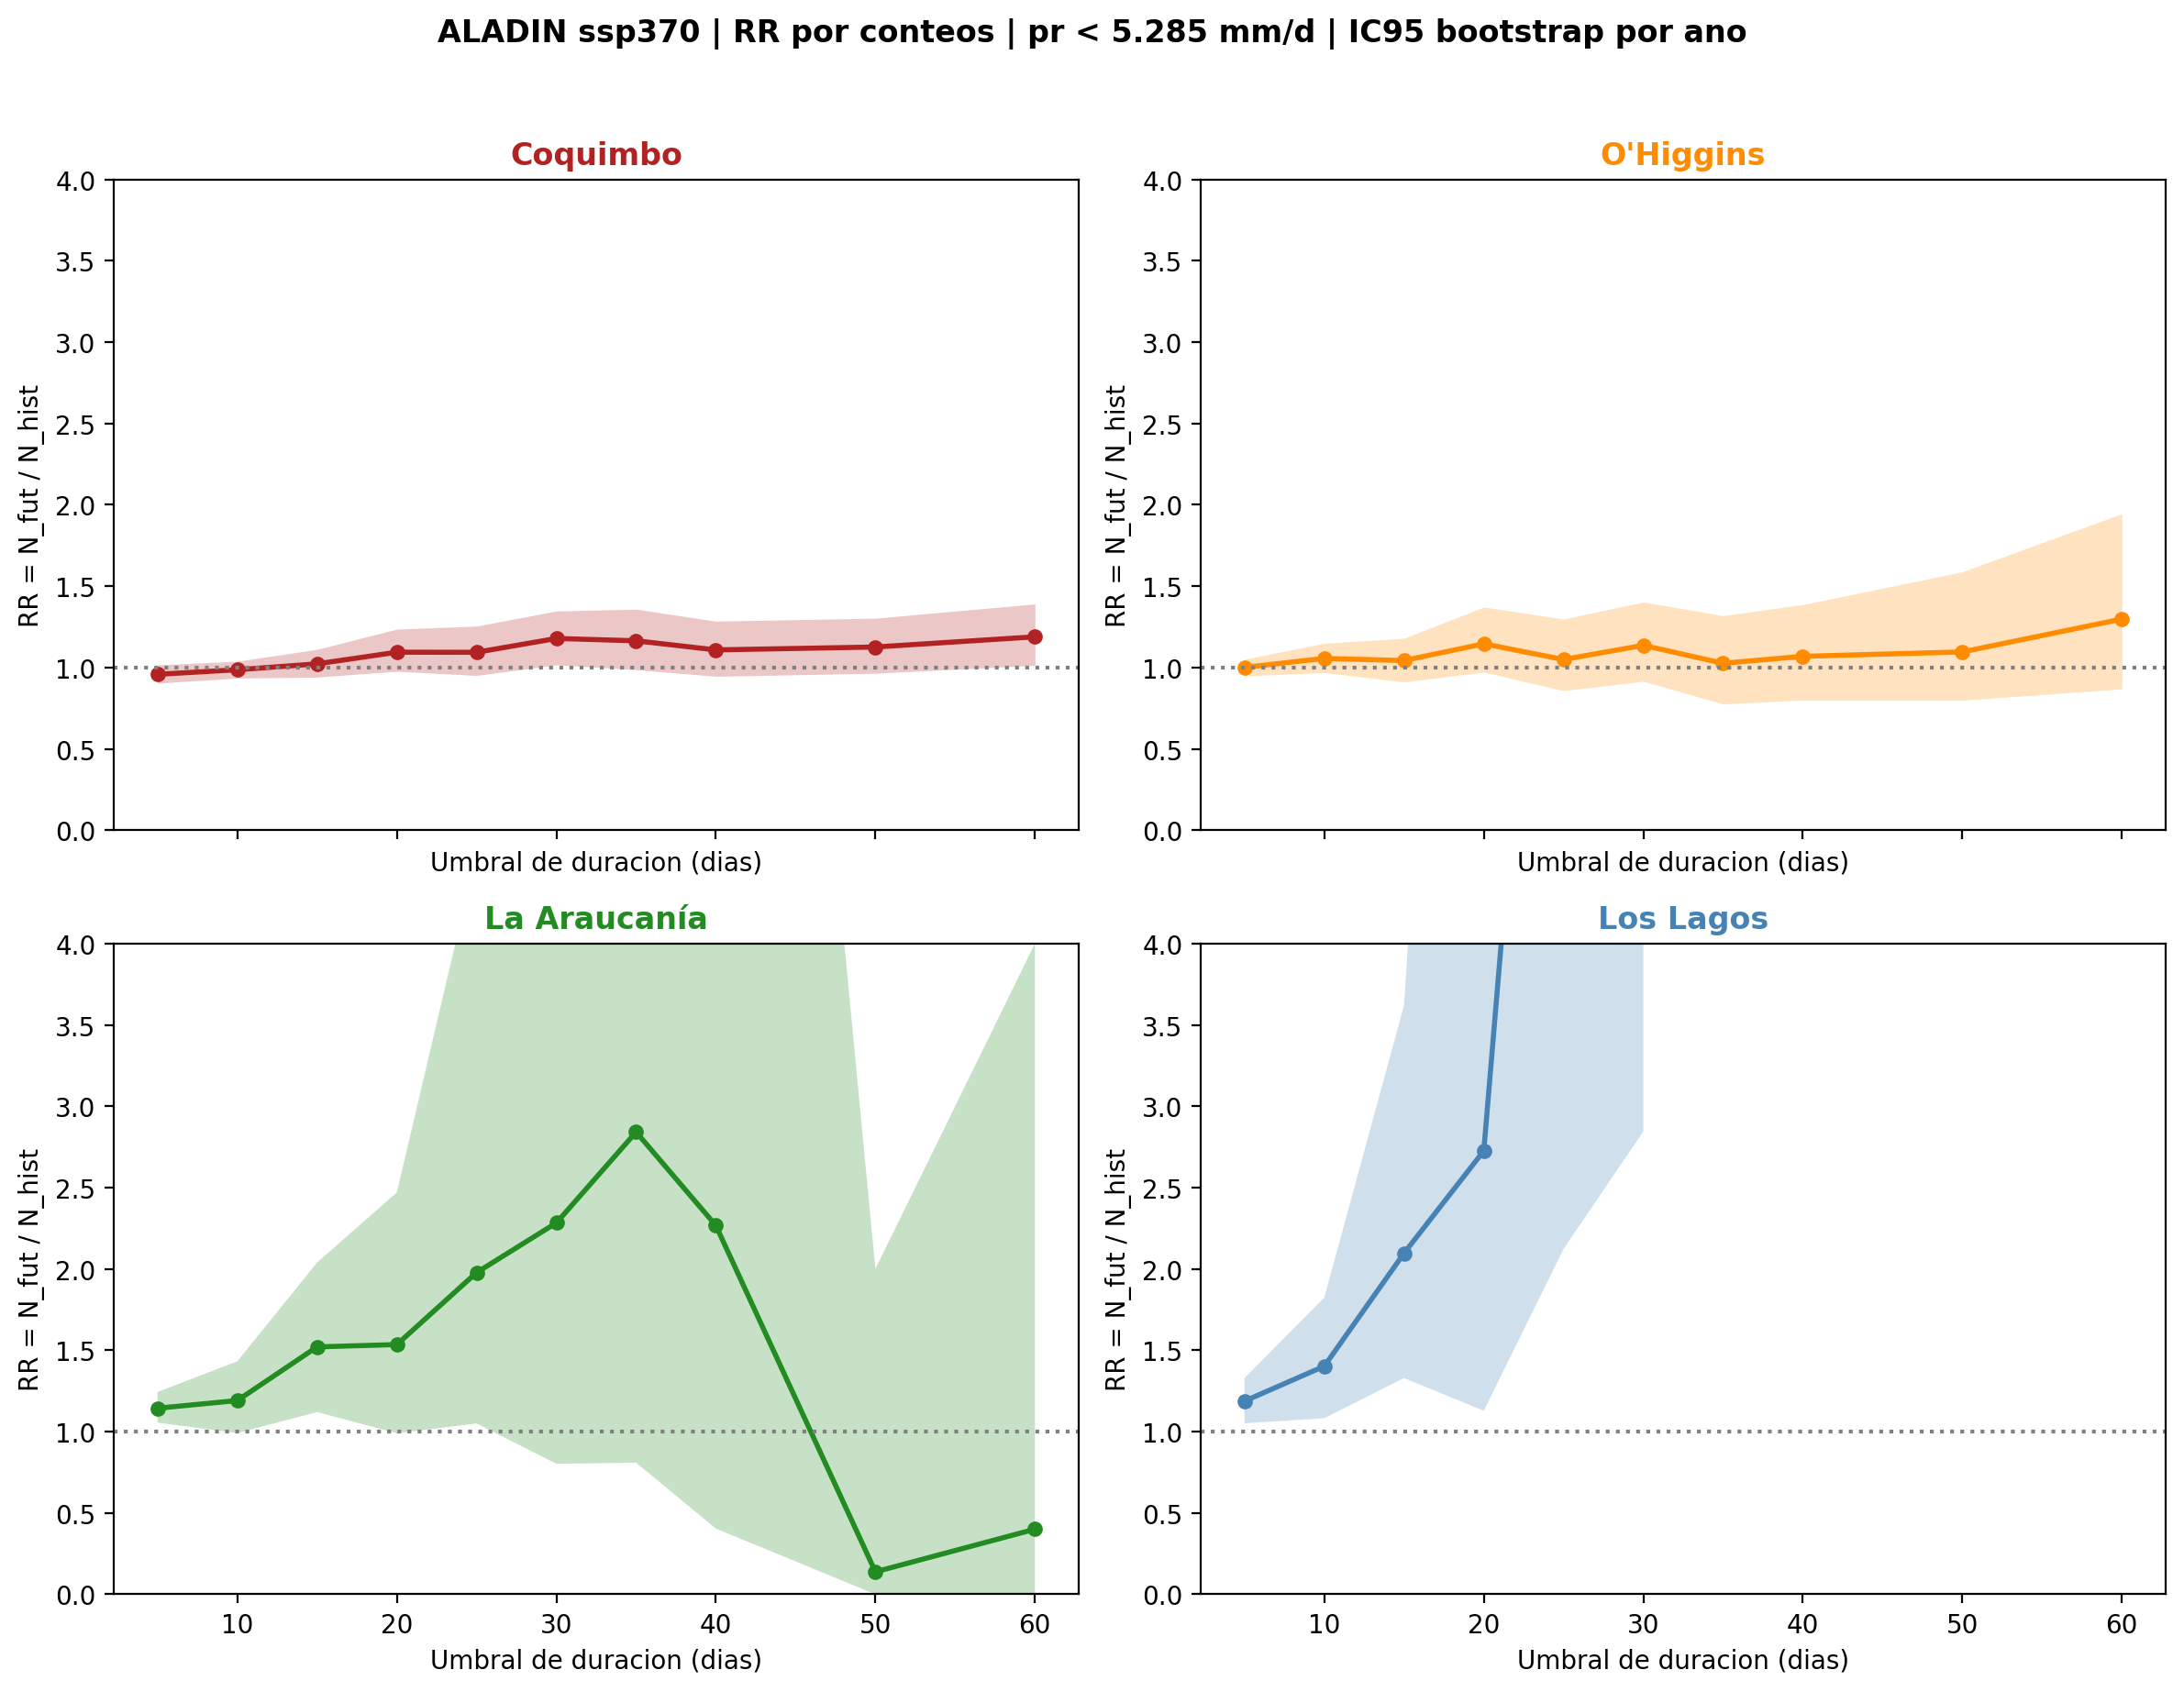
\includegraphics[width=1\linewidth,height=0.72\textheight,keepaspectratio,alt={Risk ratio RR(D) = N\_fut(t ≥ D) / N\_hist(t ≥ D) en función del umbral de duración D para las cuatro regiones, con ALADIN bajo SSP3-7.0 (2040--2074) frente al histórico (1980--2014), R₀ = 5,285 mm día$^{-1}$ y rachas iniciadas entre marzo y noviembre. La banda sombreada es el intervalo de confianza del 95 \% por bootstrap por años.}]{figS_rr_curves_aladin_ssp370.png}
\caption[Risk ratio RR(D) = N\_fut(t ≥ D) / N\_hist(t ≥ D) en función del umbral de duración D para las cuatro regiones, con ALADIN bajo SSP3-7.0 (2040--2074) frente al histórico (1980--2014), R₀ = 5,285 mm día$^{-1}$ y rachas iniciadas entre marzo y noviembre]{Risk ratio RR(D) = N\_fut(t ≥ D) / N\_hist(t ≥ D) en función del umbral de duración D para las cuatro regiones, con ALADIN bajo SSP3-7.0 (2040--2074) frente al histórico (1980--2014), R₀ = 5,285 mm día$^{-1}$ y rachas iniciadas entre marzo y noviembre. La banda sombreada es el intervalo de confianza del 95 \% por bootstrap por años.}\label{fig:S4}
\end{figure}

\chapter{Código, datos y reproducibilidad}\label{anx:B}

\pendiente{completar. Borrador de la relación entre scripts y resultados:}

{\def\LTcaptype{none} % do not increment counter
\begin{longtable}[]{@{}
  >{\raggedright\arraybackslash}p{(\linewidth - 2\tabcolsep) * \real{0.5000}}
  >{\raggedright\arraybackslash}p{(\linewidth - 2\tabcolsep) * \real{0.5000}}@{}}
\toprule\noalign{}
\begin{minipage}[b]{\linewidth}\raggedright
Resultado
\end{minipage} & \begin{minipage}[b]{\linewidth}\raggedright
Script
\end{minipage} \\
\midrule\noalign{}
\endhead
\bottomrule\noalign{}
\endlastfoot
Figura~\ref{fig:dominio} (dominio) & \texttt{\_generar\_figuras\_paper\_faltantes.py} (función \texttt{fig02\_dominio}) \\
Figura~\ref{fig:esquema} (esquema de dry spell) & \texttt{\_generar\_fig02\_esquema\_dryspell.py} \\
Figura~\ref{fig:calibracion} (calibración de R₀) & \texttt{\_generar\_fig03\_calibracion\_R0.py} \\
Figura~\ref{fig:mapas}, Tabla~\ref{tab:S1} y bootstrap de mapas & \texttt{\_run\_pregunta7\_bootstrap.py}, \texttt{\_generar\_fig32\_persistencia\_biases.py}, \texttt{\_generar\_tablaS1\_sensibilidad\_chile.py} \\
Figura~\ref{fig:pdfs} y Tabla~\ref{tab:estadisticos} & \texttt{\_generar\_pregunta9\_pdf\_loglog\_cuencas.py} \\
Figura~\ref{fig:mapas_futuro} & Sin script (pendiente) \\
Figura~\ref{fig:rr}, Tabla~\ref{tab:rr}, Tabla~\ref{tab:S3}, Figura~\ref{fig:S3}, Tabla~\ref{tab:S5} y Figura~\ref{fig:S4} & \texttt{\_run\_pregunta5\_aladin.py} (opciones \texttt{-\/-umbral} y \texttt{-\/-escenario}) \\
Figura~\ref{fig:S1} y Tabla~\ref{tab:S2} & \texttt{\_generar\_figS1\_sensibilidad\_umbral.py} \\
Figura~\ref{fig:S2} & \texttt{\_generar\_figS2\_mapa\_R0\_local.py} \\
S5 (regrillado) & \texttt{\_test\_regrillado\_conservativo.py} \\
Conteo de rachas censuradas & \texttt{\_cuantificar\_censuradas.py} \\
\end{longtable}
}

\textbf{Disponibilidad de datos (borrador).} CR2MET v2.5 está disponible públicamente en el Centro de Ciencia del Clima y la Resiliencia (CR2). Las simulaciones CNRM-ALADIN64 (dominio CHP12) fueron facilitadas por \pendiente{fuente original; preguntar al profesor} y están disponibles a solicitud.


\end{document}
